\documentclass[conference]{IEEEtran}
% Times for text and maths, as IEEE requires. T1 encoding makes IEEEtran's
% Times (ptm) work under pdfLaTeX, and also under XeTeX/Tectonic, which would
% otherwise fall back to Latin Modern ("Font shape TU/ptm undefined").
\usepackage[T1]{fontenc}
\usepackage{amsmath}
\usepackage{newtxtext,newtxmath}
\usepackage{cite}
\usepackage{graphicx}
\usepackage{booktabs}
\usepackage{array}
\usepackage{tabularx}
\usepackage{multirow}
\usepackage{url}
\usepackage{tikz}
\usetikzlibrary{arrows.meta, shapes.geometric}
\usepackage{pgfplots}
\pgfplotsset{compat=1.17}

% ---------------------------------------------------------------------------
% Team details: set these once; they are used in the author block and in the
% Individual Contributions section.
% ---------------------------------------------------------------------------
% Names confirmed by the team on 15 Nov 2026.
\newcommand{\MemA}{Kanishk}     % Member 1, GitHub kanishksharma04
\newcommand{\MemB}{Adarsh}      % Member 2, GitHub AdarshVashith
\newcommand{\MemC}{Deepanshu}   % Member 3, GitHub deepanshu-sharma425
\newcommand{\MemD}{Daksh}       % Member 4, GitHub emphor11
\newcommand{\MemE}{Ram}         % Member 5, GitHub Adrenox20
\newcommand{\Dept}{Department of Computer Science and Artificial Intelligence}
\newcommand{\Inst}{Newton School of Technology, Rishihood University, Sonipat, Haryana}

\begin{document}

\title{Instruction and Data Memory Hierarchy:\\
From a Harvard Memory Organisation to Split Caches\\over a Shared Memory}

\author{\IEEEauthorblockN{\MemA, \MemB, \MemC, \MemD, \MemE}
\IEEEauthorblockA{Modern Computer Architecture, Project 9 (Final Report, Phase II)\\
\Dept\\
\Inst}}

\maketitle

% =============================================================================
\begin{abstract}
When instructions and data share one memory port, as in the von Neumann
organisation, an instruction fetch and a load or store cannot happen in the
same cycle. A Harvard organisation removes this conflict with separate
instruction and data memories. We implement both in synthesizable Verilog
around the same single-cycle processor for a 25-instruction subset of RV32I,
and then extend the study to a realistic memory hierarchy: a
\emph{modified Harvard} system with split, direct-mapped, write-through
level-1 instruction and data caches, a write buffer and an arbiter in front
of one unified memory of configurable latency, compared with a von Neumann
system that has a single unified cache of the same capacity and with one that
has no cache. With ideal single-cycle memories, the Harvard design runs at a
CPI of exactly 1.00, while the shared-memory baseline needs 1.02 to 1.45,
i.e.\ one extra cycle per load or store. In a sweep of 104 configurations over
eight programs, all checked against an independent instruction-set and cache
model, split caches give a geometric-mean CPI of 1.47 at a memory latency of
four cycles, against 2.03 for the unified cache and 4.74 without a cache. The
unified cache loses both to its single port and to conflict misses between
code and data that map to the same cache lines; the write buffer adds up to
1.41$\times$. In synthesis for a Xilinx 7-series FPGA, the split organisation
also uses about 20\% fewer LUTs than its shared counterpart, both with ideal
memories and with caches.
\end{abstract}

\begin{IEEEkeywords}
Harvard architecture, von Neumann architecture, memory hierarchy, split cache,
unified cache, write buffer, RISC-V, Verilog, CPI
\end{IEEEkeywords}

% =============================================================================
\section{Introduction}

The stored-program concept, described in von Neumann's report on the
EDVAC~\cite{vonneumann_edvac}, keeps the program in the same kind of memory
as the data it operates on. This made computers general purpose, but it also
means that the processor must use memory for two different purposes: to fetch
its next instruction and to read or write data. If both go through the same
memory port, they compete for it. Backus called the single channel between
processor and memory the ``von Neumann bottleneck''~\cite{backus1978}, and the
growing gap between processor and memory speed later became known as the
memory wall~\cite{wulf1995}.

The Harvard organisation separates the two: instructions come from an
instruction memory and data from a data memory, each with its own address and
data paths, so a fetch and a data access can be performed in the same
cycle. Modern processors use a modified form of this idea, with split level-1
instruction and data caches in front of a unified main
memory~\cite{patterson_riscv,hennessy_quant}.

Phase~I of this project built a Harvard memory subsystem and a shared-memory
baseline around the same small processor and measured the difference with
ideal single-cycle memories. Phase~II, reported here together with Phase~I,
asks what happens when memory is not ideal. Its contributions are:
(i) an extension of the processor from 10 to 25 RV32I instructions
(shifts, comparisons, signed branches, jumps and calls, upper immediates),
with stall support in both cores;
(ii) a reusable direct-mapped, write-through, no-write-allocate cache with
a one-entry write buffer, a lower-level memory with configurable latency
and an instruction-first memory arbiter;
(iii) two complete hierarchies built from them, a modified Harvard system
with split caches and a von Neumann system with a unified cache of the same
capacity;
(iv) a Python instruction-set simulator that serves as an independent golden
model, including the expected cache misses, and a parameter sweep of 104
configurations that is checked against it; and
(v) FPGA synthesis of all four systems.

% =============================================================================
\section{Literature Review}

\subsection{Von Neumann and Harvard organisations}
In the von Neumann organisation, a single memory holds both instructions and
data and is reached through one address bus and one data
bus~\cite{vonneumann_edvac}. Its strength is flexibility: memory can be
divided between code and data in any proportion, and programs can be treated
as data. Its weakness is bandwidth: at most one memory transfer can occur per
memory cycle, so instruction fetch and data transfer are serialised, which is
exactly the bottleneck described by Backus~\cite{backus1978}. The
Harvard organisation, named after the Harvard Mark~I, uses physically
separate instruction and data memories. It doubles the available memory
bandwidth at the cost of a fixed partition between program and data storage
and extra hardware for a second set of buses~\cite{hennessy_quant}.

\subsection{Modified Harvard in practice}
Pure Harvard machines are rare in general-purpose computing, but the idea is
widespread. Many microcontrollers and digital signal processors keep program
code in on-chip flash and data in a separate SRAM, each with its own bus. In
general-purpose processors, the split appears in the cache hierarchy: the
level-1 cache is divided into an instruction cache and a data cache that can
be accessed in parallel by the pipeline, while lower levels and main memory
remain unified~\cite{patterson_riscv,hennessy_quant}. This ``modified
Harvard'' arrangement gives the bandwidth of separate paths near the core and
the flexibility of a single address space further away.

\subsection{Single-cycle and multi-cycle processors}
A single-cycle processor that executes a load in one cycle must read an
instruction and a data word in the same cycle, and therefore needs separate
instruction and data memories~\cite{patterson_riscv,harris_riscv}. A
multi-cycle processor can share one memory between instructions and data by
spending different cycles on fetch and on data access, which is the approach
taken by our baseline.

\subsection{RISC-V as a teaching ISA}
RISC-V is an open instruction set with a small base integer
ISA~\cite{riscv_isa}. Its regular encodings keep the decoder small, and it is
the ISA used by current editions of standard
textbooks~\cite{patterson_riscv,harris_riscv}. Asanovi\'{c} and Patterson
argue that an instruction set should be an open standard and give RISC-V's
free licence and simple base ISA as reasons for adopting it in research and
industry~\cite{asanovic2014free}.

\subsection{RISC-V soft processors on FPGAs}
Many RISC-V cores have been written in HDL and implemented on FPGAs.
Miyazaki \emph{et al.} describe RVCoreP, an RV32I soft processor with a
five-stage pipeline evaluated on a Xilinx Artix-7 board; they optimise the
instruction fetch unit, the ALU and the data memory to raise the clock
frequency~\cite{miyazaki2020rvcorep}. That work targets performance. Ours is
deliberately simpler: a single-cycle core without a pipeline, so that the
only variable in the comparison is the memory organisation.

\subsection{Caches, split versus unified}
Wilkes proposed a small fast ``slave'' memory that holds recently used words
of a larger, slower main memory~\cite{wilkes1965}, the idea behind every
modern cache. Smith's survey of cache memories discusses, among many design
choices, whether to split the cache into instruction and data halves or to
keep one unified cache: a unified cache of the same total size usually has a
somewhat lower miss ratio, because it balances its capacity between code and
data automatically, but a split design lets an instruction fetch and a data
access proceed in parallel~\cite{smith1982}. Hennessy and Patterson make the
same trade-off quantitative and conclude that the structural hazard of a
single port outweighs the miss-ratio advantage for pipelined
processors~\cite{hennessy_quant}. Hill and Smith classify misses as
compulsory, capacity and conflict misses and show how much of the miss ratio
of a direct-mapped cache is due to conflicts~\cite{hill1989}; Jouppi shows
that a small fully associative victim cache removes many of these conflict
misses~\cite{jouppi1990}.

\subsection{Write policies and write buffers}
A write-through cache sends every store to the next level, which keeps
memory up to date and makes the cache simple, at the cost of memory
traffic. Jouppi studies write-through and write-back caches with and without
write allocation and shows that a write buffer, which lets the processor
continue while a store is still on its way to memory, removes most of the
stall cost of write-through~\cite{jouppi1993}. Our Phase~II cache uses
exactly this combination (write-through, no-write-allocate, write buffer)
because it is the simplest correct design for a system with a single lower
level, and we measure the effect of the buffer directly.

% =============================================================================
\section{Proposed Solution}

\subsection{Overview: four organisations, one processor}
Table~\ref{tab:systems} lists the four systems. All of them run the same
machine code, use the same data address map and the same performance
counters, and reuse the same register file, ALU, immediate generator and
control decoder, so that the memory organisation is the only difference
between them.

\begin{table}[t]
\caption{The four organisations compared}
\label{tab:systems}
\centering
\footnotesize
\setlength{\tabcolsep}{3pt}
\begin{tabularx}{\columnwidth}{@{}>{\raggedright\arraybackslash}p{0.21\columnwidth}>{\raggedright\arraybackslash}X>{\raggedright\arraybackslash}p{0.07\columnwidth}@{}}
\toprule
Name & Organisation & Phase \\
\midrule
H (\texttt{harvard\_top}) & single-cycle core, separate instruction ROM and data RAM, both single-cycle & I \\
VN (\texttt{vn\_top}) & two-state core, one single-cycle memory for code and data & I \\
MH (\texttt{mh\_top}) & single-cycle core with stall, split I-cache and D-cache, arbiter, one unified memory of latency $L$ & II \\
UC (\texttt{vnc\_top}) & two-state core with stall, one unified cache of the same total size, same memory & II \\
NC (\texttt{vnc\_top}) & two-state core with stall, no cache, same memory & II \\
\bottomrule
\end{tabularx}
\end{table}

\begin{figure*}[t]
\centering
% Block diagram: Harvard system (left) vs shared-memory baseline (right)
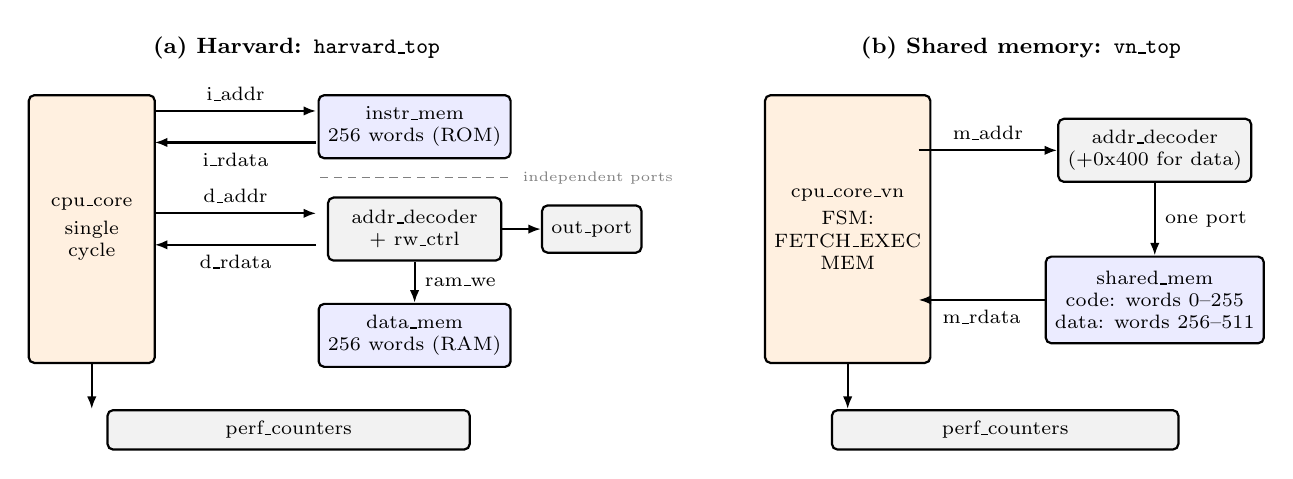
\begin{tikzpicture}[
    font=\scriptsize,
    blk/.style={draw, thick, rounded corners=2pt, align=center, minimum height=0.8cm},
    mem/.style={blk, fill=blue!8},
    cpu/.style={blk, fill=orange!12},
    misc/.style={blk, fill=gray!10},
    bus/.style={-{Latex[length=1.6mm]}, thick},
    x=1cm, y=1cm]

% ---------------- (a) Harvard ----------------
\node[font=\footnotesize\bfseries] at (2.6,3.2) {(a) Harvard: \texttt{harvard\_top}};
\node[cpu, minimum width=1.6cm, minimum height=3.4cm] (core) at (0,0.9) {cpu\_core\\[2pt]single\\cycle};

\node[mem, minimum width=2.2cm] (imem) at (4.1,2.2) {instr\_mem\\256 words (ROM)};
\node[misc, minimum width=2.2cm] (dec) at (4.1,0.9) {addr\_decoder\\+ rw\_ctrl};
\node[mem, minimum width=2.2cm] (dmem) at (4.1,-0.45) {data\_mem\\256 words (RAM)};
\node[misc, minimum width=1.0cm, minimum height=0.6cm] (out) at (6.35,0.9) {out\_port};

\draw[bus] (0.8,2.4) -- node[above]{i\_addr} (2.85,2.4);
\draw[bus] (2.85,2.0) -- node[below]{i\_rdata} (0.8,2.0);
\draw[bus] (0.8,1.1) -- node[above]{d\_addr} (2.85,1.1);
\draw[bus] (2.85,0.7) -- node[below]{d\_rdata} (0.8,0.7);
\draw[bus] (dec.south) -- node[right]{ram\_we} (dmem.north);
\draw[bus] (dec.east) -- (out.west);
\draw[densely dashed, gray] (2.9,1.55) -- (5.3,1.55);
\node[gray, font=\tiny, anchor=west] at (5.35,1.55) {independent ports};

\node[misc, minimum width=4.6cm, minimum height=0.5cm] (perf) at (2.5,-1.65) {perf\_counters};
\draw[bus] (core.south) -- (core.south |- perf.north);

% ---------------- (b) Shared memory ----------------
\begin{scope}[xshift=9.6cm]
\node[font=\footnotesize\bfseries] at (2.2,3.2) {(b) Shared memory: \texttt{vn\_top}};
\node[cpu, minimum width=1.8cm, minimum height=3.4cm] (vcore) at (0,0.9) {cpu\_core\_vn\\[2pt]FSM:\\FETCH\_EXEC\\MEM};
\node[misc, minimum width=2.2cm] (vdec) at (3.9,1.9) {addr\_decoder\\(+0x400 for data)};
\node[mem, minimum width=2.2cm, minimum height=1.1cm] (sm) at (3.9,0.0) {shared\_mem\\code: words 0--255\\data: words 256--511};

\draw[bus] (0.9,1.9) -- node[above]{m\_addr} (vdec.west);
\draw[bus] (vdec.south) -- node[right]{one port} (sm.north);
\draw[bus] (sm.west) -- node[below]{m\_rdata} (0.9,0.0);

\node[misc, minimum width=4.4cm, minimum height=0.5cm] (vperf) at (2.0,-1.65) {perf\_counters};
\draw[bus] (vcore.south) -- (vcore.south |- vperf.north);
\end{scope}
\end{tikzpicture}

\caption{Phase I. (a) Harvard system: the instruction port and the data port reach separate memories, so a fetch and a load/store happen in the same cycle. (b) Shared-memory baseline: one port carries both fetches and data accesses.}
\label{fig:block}
\end{figure*}

\subsection{Memory map}
The instruction memory holds 256 words (byte addresses \texttt{0x000}--\texttt{0x3FF}).
The data address space is shown in Table~\ref{tab:map}. Wherever code and
data share one physical memory (VN, MH, UC, NC), that memory holds code in
words 0--255 and data in words 256--511; the top level adds \texttt{0x400} to
data RAM addresses, so the same program and data images run unmodified on all
designs. The output register and invalid addresses never reach a memory or a
cache.

\begin{table}[t]
\caption{Data address map (all designs)}
\label{tab:map}
\centering
\begin{tabular}{ll}
\toprule
Byte address & Region \\
\midrule
\texttt{0x000}--\texttt{0x3FF} & Data RAM, 256 words \\
\texttt{0x400} & \texttt{out\_port} register (write-only, reads 0) \\
other & invalid: write ignored, read 0, \texttt{d\_fault}=1 \\
\bottomrule
\end{tabular}
\end{table}

\subsection{Harvard memory subsystem (Phase I)}
The \texttt{harvard\_mem} module contains four blocks. The instruction memory
is a read-only array with combinational read. The data memory is a RAM with
synchronous write and combinational read. The address decoder compares the
data address against the map and asserts exactly one of \texttt{sel\_ram},
\texttt{sel\_io} or \texttt{addr\_fault}. The read/write controller turns the
processor's requests into a RAM write enable or an \texttt{out\_port} write
enable and selects the read data. The instruction port and the data port
share no address bus, data bus or array, so a fetch and a data access
complete in the same cycle (Fig.~\ref{fig:block}a).

\subsection{Processor and instruction-set extension}
The processor is single-cycle: in one clock period it fetches the instruction
at the program counter, decodes it, reads two registers, computes a result,
address or branch condition in the ALU, performs the data access for LW or
SW, and writes the result back (Fig.~\ref{fig:datapath}). Phase~I supported
ADD, SUB, AND, OR, ADDI, LW, SW, BEQ, BNE and EBREAK. Phase~II adds XOR, SLT,
SLL, SRL and their immediate forms, BLT and BGE, JAL and JALR, and LUI, all
encoded as in RV32I~\cite{riscv_isa}. The ALU gained XOR, a signed
set-less-than and two shifts while keeping a 3-bit operation code; BLT and
BGE use the ALU's set-less-than output in the same way that BEQ and BNE use
its zero flag. The write-back multiplexer gained two inputs, PC$+4$ for the
link register of JAL and JALR and the immediate for LUI, and the next-PC
logic gained the jump targets. These instructions make it possible to write
programs with nested loops, signed comparisons and subroutine calls.

\begin{figure}[t]
\centering
\resizebox{\columnwidth}{!}{% Single-cycle datapath of cpu_core (Harvard). Highlighted (red): the LW path.
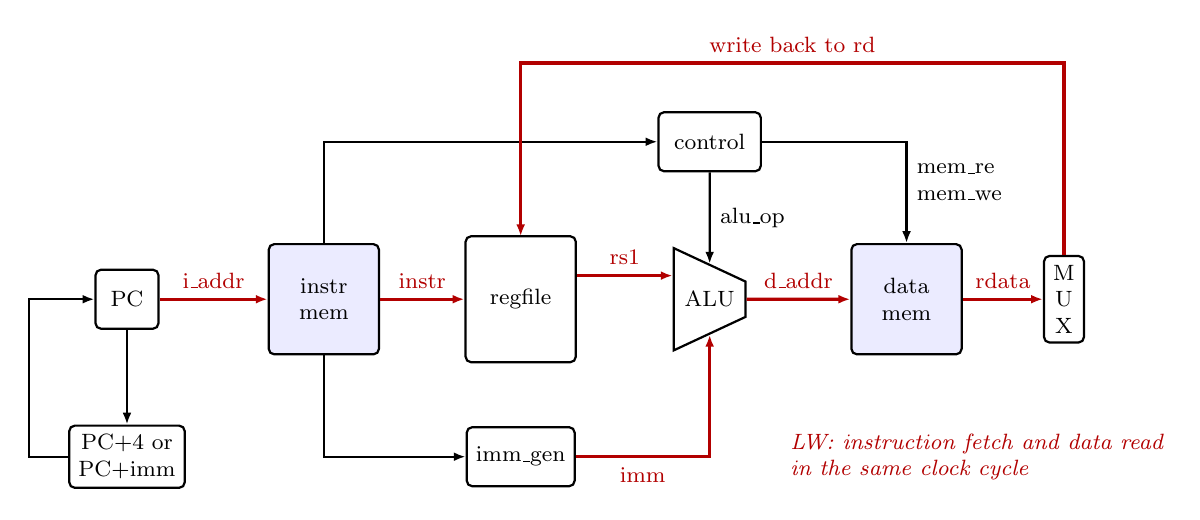
\begin{tikzpicture}[
    font=\footnotesize,
    blk/.style={draw, thick, rounded corners=2pt, align=center, minimum height=0.75cm, fill=white},
    mem/.style={blk, fill=blue!8},
    bus/.style={-{Latex[length=1.5mm]}, thick},
    lw/.style={bus, red!70!black, line width=1.1pt},
    x=1cm, y=1cm]

\node[blk, minimum width=0.8cm] (pc) at (0,0) {PC};
\node[mem, minimum width=1.4cm, minimum height=1.4cm] (imem) at (2.5,0) {instr\\mem};
\node[blk, minimum width=1.4cm, minimum height=1.6cm] (rf) at (5.0,0) {regfile};
\node[draw, thick, trapezium, trapezium left angle=65, trapezium right angle=65,
      shape border rotate=270, minimum width=1.3cm, minimum height=0.7cm, fill=white] (alu) at (7.4,0) {ALU};
\node[mem, minimum width=1.4cm, minimum height=1.4cm] (dmem) at (9.9,0) {data\\mem};
\node[blk, minimum width=0.5cm, minimum height=1.1cm] (mux) at (11.9,0) {M\\U\\X};
\node[blk, minimum width=1.3cm] (ctrl) at (7.4,2.0) {control};
\node[blk, minimum width=1.3cm] (imm) at (5.0,-2.0) {imm\_gen};
\node[blk, minimum width=1.3cm] (nextpc) at (0,-2.0) {PC+4 or\\PC+imm};

% fetch
\draw[lw] (pc.east) -- node[above]{i\_addr} (imem.west);
\draw[lw] (imem.east) -- node[above]{instr} (rf.west);
\draw[bus] (imem.north) |- (ctrl.west);
\draw[bus] (imem.south) |- (imm.west);
% execute
\draw[lw] ([yshift=3mm]rf.east) -- node[above]{rs1} ([yshift=3mm]rf.east -| alu.west);
\draw[lw] (imm.east) -| node[pos=0.25, below]{imm} (alu.south);
\draw[bus] (ctrl.south) -- node[right]{alu\_op} (alu.north);
\draw[bus] (ctrl.east) -| node[pos=0.7, right, align=left]{mem\_re\\mem\_we} (dmem.north);
% memory and write back
\draw[lw] (alu.east) -- node[above]{d\_addr} (dmem.west);
\draw[lw] (dmem.east) -- node[above]{rdata} (mux.west);
\draw[lw] (mux.north) |- (11.9,3.0) -| node[pos=0.25, above]{write back to rd} (5.0,0.8);
% next PC
\draw[bus] (pc.south) -- (nextpc.north);
\draw[bus] (nextpc.west) -- ++(-0.5,0) |- (pc.west);

\node[red!70!black, font=\footnotesize\itshape, align=left, anchor=west] at (8.3,-2.0)
    {LW: instruction fetch and data read\\in the same clock cycle};
\end{tikzpicture}
}
\caption{Single-cycle datapath of \texttt{cpu\_core} (Phase I instruction subset shown). The highlighted path is an LW, which uses the instruction memory and the data memory in the same cycle. Phase II adds PC$+4$ and immediate inputs to the write-back multiplexer, jump targets to the next-PC logic, and a stall input.}
\label{fig:datapath}
\end{figure}

For Phase~II the core also gained two inputs, \texttt{i\_ready} and
\texttt{d\_ready}. When \texttt{i\_ready} is low, no valid instruction is
available: the core decodes a NOP in its place and holds its state. When a
load or store is pending and \texttt{d\_ready} is low, the core holds the
program counter and does not write the register file. During a stall all of
the core's outputs stay constant, so the memory side sees a stable request.
The Phase~I top level ties both inputs high, which gives cycle-identical
Phase~I behaviour; the Phase~I regression confirms this.

\subsection{Shared-memory baseline}
The baseline processor has a single memory bus driven by a two-state
controller (Fig.~\ref{fig:fsm}). In the \textsc{FetchExec} state the bus
carries the program counter; arithmetic, branch, jump and EBREAK
instructions complete in this state. A load or store cannot use the bus a
second time, so the instruction is latched and the controller moves to the
\textsc{Mem} state, where the bus carries the data address. Loads and stores
therefore take two cycles and all other instructions one. For Phase~II this
core gained a \texttt{m\_ready} input: when the bus transfer of the current
cycle has not finished, it holds its state, PC and latched instruction.

\begin{figure}[t]
\centering
% Two-state controller of cpu_core_vn (shared-memory baseline)
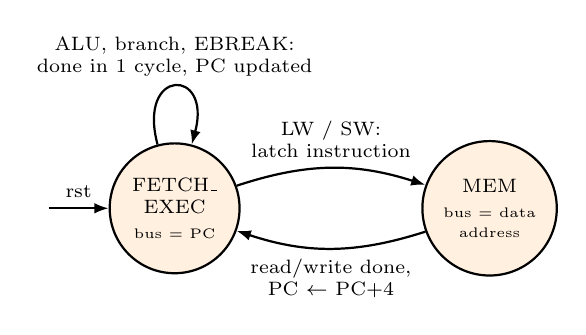
\begin{tikzpicture}[
    font=\scriptsize,
    st/.style={draw, thick, circle, minimum size=1.6cm, align=center, fill=orange!12},
    tr/.style={-{Latex[length=1.8mm]}, thick},
    x=1cm, y=1cm]
\node[st] (fe) at (0,0) {FETCH\_\\EXEC\\[1pt]\tiny bus = PC};
\node[st] (mem) at (4,0) {MEM\\[1pt]\tiny bus = data\\[-1pt]\tiny address};
\draw[tr] (-1.6,0) -- node[above]{rst} (fe.west);
\draw[tr] (fe) edge[loop above, looseness=6] node[above, align=center]
    {ALU, branch, EBREAK:\\done in 1 cycle, PC updated} (fe);
\draw[tr] (fe.20) to[bend left=18] node[above, align=center]{LW / SW:\\latch instruction} (mem.160);
\draw[tr] (mem.200) to[bend left=18] node[below, align=center]{read/write done,\\PC $\leftarrow$ PC+4} (fe.340);
\end{tikzpicture}

\caption{Two-state controller of the shared-memory baseline.}
\label{fig:fsm}
\end{figure}

\subsection{Phase II: the memory hierarchy}
Fig.~\ref{fig:hier} shows the two Phase~II systems. They are built from
three new modules.

\begin{figure*}[t]
\centering
\resizebox{\textwidth}{!}{% Phase II block diagram: modified Harvard (left) vs von Neumann with a unified cache (right)
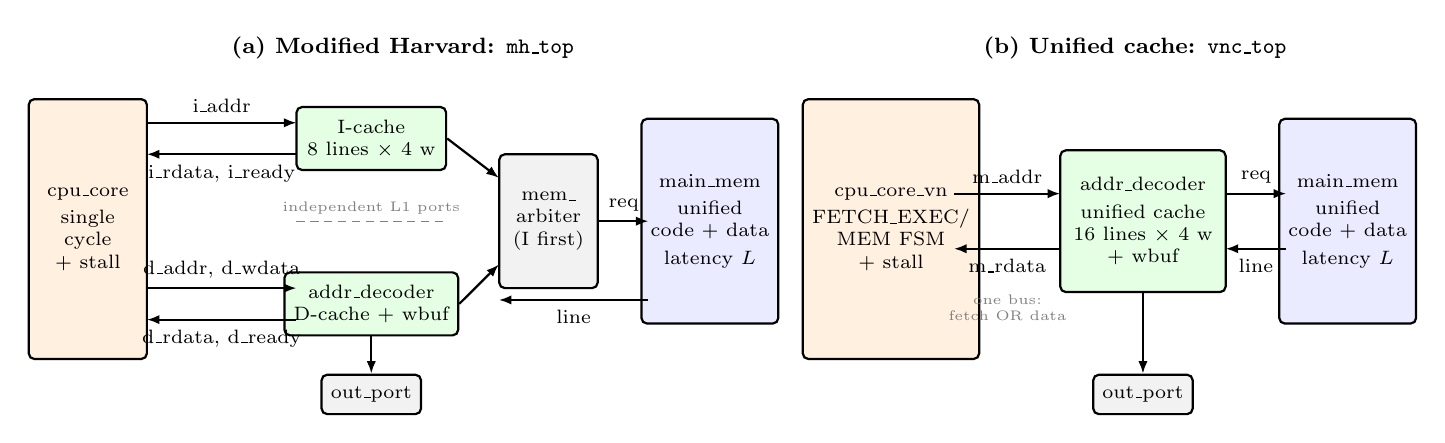
\begin{tikzpicture}[
    font=\scriptsize,
    blk/.style={draw, thick, rounded corners=2pt, align=center, minimum height=0.8cm},
    mem/.style={blk, fill=blue!8},
    cch/.style={blk, fill=green!10},
    cpu/.style={blk, fill=orange!12},
    misc/.style={blk, fill=gray!10},
    bus/.style={-{Latex[length=1.6mm]}, thick},
    x=1cm, y=1cm]

% ---------------- (a) modified Harvard ----------------
\node[font=\footnotesize\bfseries] at (4.0,2.85) {(a) Modified Harvard: \texttt{mh\_top}};
\node[cpu, minimum width=1.5cm, minimum height=3.3cm] (core) at (0,0.55) {cpu\_core\\[2pt]single\\cycle\\+ stall};

\node[cch, minimum width=1.9cm] (ic) at (3.6,1.7) {I-cache\\8 lines $\times$ 4 w};
\node[cch, minimum width=1.9cm] (dc) at (3.6,-0.4) {addr\_decoder\\D-cache + wbuf};
\node[misc, minimum width=1.0cm, minimum height=0.5cm] (out) at (3.6,-1.55) {out\_port};
\node[misc, minimum width=1.25cm, minimum height=1.7cm] (arb) at (5.85,0.65) {mem\_\\arbiter\\(I first)};
\node[mem, minimum width=1.55cm, minimum height=2.6cm] (mm) at (7.9,0.65) {main\_mem\\[2pt]unified\\code + data\\[2pt]latency $L$};

\draw[bus] (0.75,1.9) -- node[above]{i\_addr} (2.65,1.9);
\draw[bus] (2.65,1.5) -- node[below]{i\_rdata, i\_ready} (0.75,1.5);
\draw[bus] (0.75,-0.2) -- node[above]{d\_addr, d\_wdata} (2.65,-0.2);
\draw[bus] (2.65,-0.6) -- node[below]{d\_rdata, d\_ready} (0.75,-0.6);
\draw[bus] (dc.south) -- (out.north);
\draw[bus] (ic.east) -- (5.22,1.2);
\draw[bus] (dc.east) -- (5.22,0.1);
\draw[bus] (arb.east) -- node[above]{req} (7.12,0.65);
\draw[bus] (7.12,-0.35) -- node[below]{line} (5.22,-0.35);
\draw[densely dashed, gray] (2.65,0.65) -- (4.55,0.65);
\node[gray, font=\tiny] at (3.6,0.82) {independent L1 ports};

% ---------------- (b) von Neumann + unified cache ----------------
\node[font=\footnotesize\bfseries] at (13.3,2.85) {(b) Unified cache: \texttt{vnc\_top}};
\node[cpu, minimum width=1.6cm, minimum height=3.3cm] (vcore) at (10.2,0.55) {cpu\_core\_vn\\[2pt]FETCH\_EXEC/\\MEM FSM\\+ stall};
\node[cch, minimum width=2.1cm, minimum height=1.8cm] (uc) at (13.4,0.65) {addr\_decoder\\[2pt]unified cache\\16 lines $\times$ 4 w\\+ wbuf};
\node[misc, minimum width=1.0cm, minimum height=0.5cm] (vout) at (13.4,-1.55) {out\_port};
\node[mem, minimum width=1.55cm, minimum height=2.6cm] (vmm) at (16.0,0.65) {main\_mem\\[2pt]unified\\code + data\\[2pt]latency $L$};

\draw[bus] (11.0,1.0) -- node[above]{m\_addr} (12.35,1.0);
\draw[bus] (12.35,0.3) -- node[below]{m\_rdata} (11.0,0.3);
\draw[bus] (uc.south) -- (vout.north);
\draw[bus] (14.45,1.0) -- node[above]{req} (15.22,1.0);
\draw[bus] (15.22,0.3) -- node[below]{line} (14.45,0.3);
\node[gray, font=\tiny, align=center] at (11.68,-0.45) {one bus:\\fetch OR data};
\end{tikzpicture}
}
\caption{Phase II. (a) Modified Harvard: split level-1 caches keep the Harvard property near the core, while a single memory below them holds code and data. (b) Von Neumann with one unified cache of the same total capacity in front of the same memory.}
\label{fig:hier}
\end{figure*}

\emph{Cache} (\texttt{cache.v}). A direct-mapped cache, parameterised by the
number of lines and the words per line (four in all experiments). A read
that hits completes in the same cycle. A read miss requests the whole line
from memory, writes it into the cache when memory answers, and completes on
the next cycle as a hit, so the miss penalty is exactly $L$ cycles. Stores
are write-through and no-write-allocate: a store that hits also updates the
cached word, a store that misses does not bring the line in. With the write
buffer enabled, a store is placed in a one-entry buffer and completes at
once if the buffer is empty or is being drained in that very cycle;
otherwise the core waits. A read miss waits until the buffer is empty, so
memory is always up to date before a line is fetched and no read-after-write
hazard is possible. The same module serves as I-cache (it never sees a
store), D-cache and unified cache; with caching disabled it becomes an
uncached path that forwards each memory word to the core.

\emph{Lower-level memory} (\texttt{main\_mem.v}). One 512-word memory with a
request/ready handshake and a fixed access time: \texttt{ready} is high in
the $L$-th cycle of a request, so $L=1$ is the ideal single-cycle memory of
Phase~I. A read returns the full four-word line in one transfer.

\emph{Arbiter} (\texttt{mem\_arbiter.v}). In MH, the I-cache and the D-cache
share the memory. Instruction requests have priority, and a transfer that
has started keeps the memory until it completes. Because the core is
single-cycle, the D-cache can only miss while the I-cache hits, so the only
real conflict is an I-cache miss that arrives while the write buffer is
draining; the arbiter counts these cycles.

\emph{Timing design.} Two design rules keep MH free of combinational loops,
which matters for both simulation and timing analysis. First, the caches do
not forward the missing word to the core during the refill cycle: forwarding
would create the path memory $\rightarrow$ instruction $\rightarrow$ data
address $\rightarrow$ arbiter $\rightarrow$ memory. Second, the memory's
\texttt{ready} and the arbiter's idle grant depend only on registered state,
not on the other side's request. One loop was found the hard way: with a
one-line I-cache, deriving the I-cache read enable from \texttt{halt} closed
the loop \texttt{i\_ready} $\rightarrow$ instruction $\rightarrow$
\texttt{halt} $\rightarrow$ read enable $\rightarrow$ \texttt{i\_ready}, and
the simulator oscillated when a stale EBREAK sat in the missing line. The
read enable is now constant. Yosys confirms that MH has no logic loop; UC
inherits the structural false loop of the Phase~I baseline.

\subsection{Verification}
Verification has four layers, all self-checking.
(1) A two-pass assembler, whose self-test now checks 29 encodings, including
reference encodings such as \texttt{ret}~$=$~\texttt{0x00008067}.
(2) A Python instruction-set simulator (\texttt{iss.py}), written
independently of the RTL, that executes a program image and predicts the
final registers and memory, the dynamic instruction and load/store counts,
and the number of misses of split and unified direct-mapped caches of any
size.
(3) Unit testbenches for the decoder, memories and \texttt{harvard\_mem}, and
a directed cache test that checks miss timing ($L{+}1$ cycles including the
hit), hits, buffered stores, a store waiting for a busy buffer,
no-write-allocate, conflict eviction and the uncached mode.
(4) System testbenches. The Phase~I comparison testbench runs H and VN side by
side and checks that VN cycles equal H cycles plus loads and stores. The
Phase~II testbench runs H, MH, UC and NC on the same program and checks that
all 32 registers, all 256 data words and the output register agree with H,
that instruction counts agree, and that every cycle is accounted for (MH:
cycles $=$ instructions $+$ I-stall $+$ D-stall cycles; UC, NC: cycles $=$
bus cycles $+$ stall cycles). With $L=1$ and no cache, NC must reproduce the
Phase~I baseline cycle for cycle. Finally, a sweep script runs 104
configurations (8 programs $\times$ latencies 1--16, cache sizes 1--32
lines, write buffer on/off) and compares every RTL miss count with the
ISS prediction. Every check passes. The design is written in
Verilog-2001~\cite{ieee1364} and simulated with Icarus Verilog.

The eight programs are: \texttt{basic} (every Phase~I instruction once),
\texttt{array\_sum}, \texttt{memcopy} and \texttt{count\_loop} from Phase~I,
and four Phase~II programs: \texttt{isa\_test} (every new instruction once),
\texttt{bubble\_sort} (16 signed words, 826 instructions, 45\% loads and
stores), \texttt{func\_call} (sum of squares through a shift-and-add multiply
subroutine called with JAL/JALR) and \texttt{transpose} (an $8\times8$ matrix
transpose followed by a row sum).

% =============================================================================
\section{Results and Discussion}

\subsection{Ideal memories: Harvard versus shared memory}
Table~\ref{tab:results} repeats the Phase~I comparison for all eight
programs. The Harvard design achieves a CPI of exactly 1.00 on every program,
and every one of its data accesses overlaps an instruction fetch. On the
baseline, each load or store adds one cycle, so CPI~$=1+f$, where $f$ is the
fraction of loads and stores; the benefit of the Harvard organisation grows
with the memory intensity of the program, from 1.02$\times$ for a
register-only loop to 1.45$\times$ for \texttt{bubble\_sort}.

\begin{table}[t]
\caption{Ideal single-cycle memories (Icarus Verilog)}
\label{tab:results}
\centering
\setlength{\tabcolsep}{3pt}
\begin{tabular}{lrrrrrrr}
\toprule
Program & Instr & LS\% & \multicolumn{2}{c}{Harvard} & \multicolumn{2}{c}{Baseline} & Simul. \\
 & & & Cyc & CPI & Cyc & CPI & cycles \\
\midrule
basic        &  19 & 36.8 &  19 & 1.00 &   26 & 1.37 &   7 \\
array\_sum   &  38 & 26.3 &  38 & 1.00 &   48 & 1.26 &  10 \\
memcopy      &  54 & 31.5 &  54 & 1.00 &   71 & 1.31 &  17 \\
count\_loop  &  64 &  1.6 &  64 & 1.00 &   65 & 1.02 &   1 \\
isa\_test    &  38 & 13.2 &  38 & 1.00 &   43 & 1.13 &   5 \\
bubble\_sort & 826 & 44.7 & 826 & 1.00 & 1195 & 1.45 & 369 \\
func\_call   & 268 &  4.1 & 268 & 1.00 &  279 & 1.04 &  11 \\
transpose    & 769 & 17.9 & 769 & 1.00 &  907 & 1.18 & 138 \\
\bottomrule
\end{tabular}
\end{table}

\subsection{Timing behaviour}
Fig.~\ref{fig:wave} is generated directly from the simulation trace of
\texttt{memcopy} with ideal memories. In cycles 4 and 5 the Harvard design
fetches an instruction and performs a load, then a store, in the same cycle;
the baseline needs cycles 4--7 for the same two instructions.

\begin{figure*}[t]
\centering
% generated by tools/vcd2tikz.py from tb_compare_memcopy.vcd -- do not edit
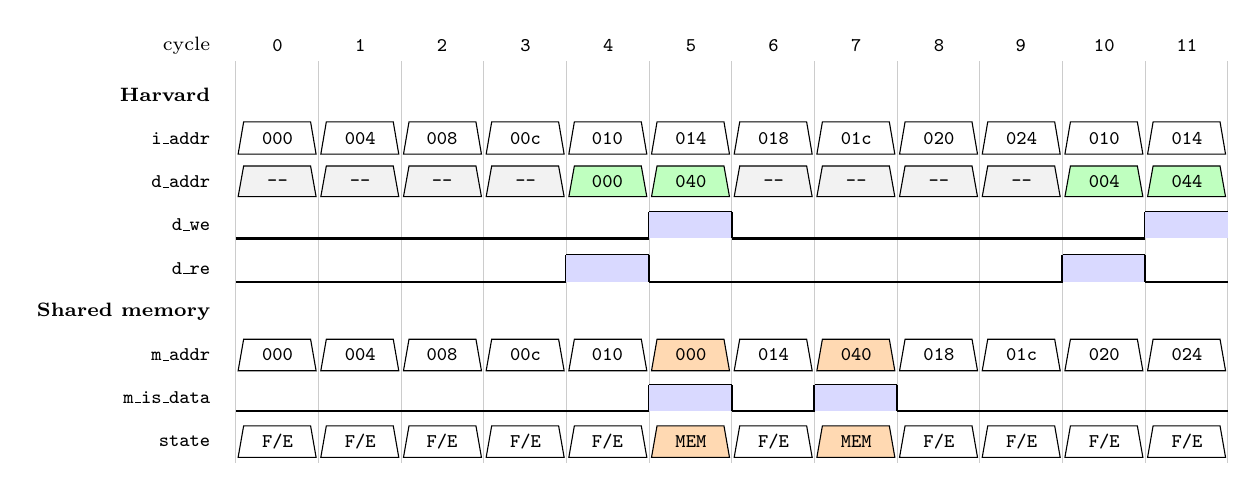
\begin{tikzpicture}[font=\scriptsize\ttfamily, x=1cm, y=1cm]
\node at (0.53,0.35) {0};
\node at (1.58,0.35) {1};
\node at (2.62,0.35) {2};
\node at (3.68,0.35) {3};
\node at (4.73,0.35) {4};
\node at (5.78,0.35) {5};
\node at (6.83,0.35) {6};
\node at (7.88,0.35) {7};
\node at (8.93,0.35) {8};
\node at (9.97,0.35) {9};
\node at (11.03,0.35) {10};
\node at (12.08,0.35) {11};
\node[anchor=east] at (-0.2,0.35) {\normalfont cycle};
\draw[gray!40] (0.00,0.15) -- (0.00,-4.95);
\draw[gray!40] (1.05,0.15) -- (1.05,-4.95);
\draw[gray!40] (2.10,0.15) -- (2.10,-4.95);
\draw[gray!40] (3.15,0.15) -- (3.15,-4.95);
\draw[gray!40] (4.20,0.15) -- (4.20,-4.95);
\draw[gray!40] (5.25,0.15) -- (5.25,-4.95);
\draw[gray!40] (6.30,0.15) -- (6.30,-4.95);
\draw[gray!40] (7.35,0.15) -- (7.35,-4.95);
\draw[gray!40] (8.40,0.15) -- (8.40,-4.95);
\draw[gray!40] (9.45,0.15) -- (9.45,-4.95);
\draw[gray!40] (10.50,0.15) -- (10.50,-4.95);
\draw[gray!40] (11.55,0.15) -- (11.55,-4.95);
\draw[gray!40] (12.60,0.15) -- (12.60,-4.95);
\node[anchor=east,font=\normalfont\bfseries\scriptsize] at (-0.2,-0.28) {Harvard};
\node[anchor=east] at (-0.2,-0.83) {i\_addr};
\draw[fill=white] (0.03,-1.03) -- (0.10,-0.62) -- (0.95,-0.62) -- (1.02,-1.03) -- cycle;
\node at (0.53,-0.83) {000};
\draw[fill=white] (1.08,-1.03) -- (1.15,-0.62) -- (2.00,-0.62) -- (2.07,-1.03) -- cycle;
\node at (1.58,-0.83) {004};
\draw[fill=white] (2.13,-1.03) -- (2.20,-0.62) -- (3.05,-0.62) -- (3.12,-1.03) -- cycle;
\node at (2.62,-0.83) {008};
\draw[fill=white] (3.18,-1.03) -- (3.25,-0.62) -- (4.10,-0.62) -- (4.17,-1.03) -- cycle;
\node at (3.68,-0.83) {00c};
\draw[fill=white] (4.23,-1.03) -- (4.30,-0.62) -- (5.15,-0.62) -- (5.22,-1.03) -- cycle;
\node at (4.72,-0.83) {010};
\draw[fill=white] (5.28,-1.03) -- (5.35,-0.62) -- (6.20,-0.62) -- (6.27,-1.03) -- cycle;
\node at (5.78,-0.83) {014};
\draw[fill=white] (6.33,-1.03) -- (6.40,-0.62) -- (7.25,-0.62) -- (7.32,-1.03) -- cycle;
\node at (6.83,-0.83) {018};
\draw[fill=white] (7.38,-1.03) -- (7.45,-0.62) -- (8.30,-0.62) -- (8.37,-1.03) -- cycle;
\node at (7.88,-0.83) {01c};
\draw[fill=white] (8.43,-1.03) -- (8.50,-0.62) -- (9.35,-0.62) -- (9.42,-1.03) -- cycle;
\node at (8.93,-0.83) {020};
\draw[fill=white] (9.48,-1.03) -- (9.55,-0.62) -- (10.40,-0.62) -- (10.47,-1.03) -- cycle;
\node at (9.98,-0.83) {024};
\draw[fill=white] (10.53,-1.03) -- (10.60,-0.62) -- (11.45,-0.62) -- (11.52,-1.03) -- cycle;
\node at (11.03,-0.83) {010};
\draw[fill=white] (11.58,-1.03) -- (11.65,-0.62) -- (12.50,-0.62) -- (12.57,-1.03) -- cycle;
\node at (12.08,-0.83) {014};
\node[anchor=east] at (-0.2,-1.38) {d\_addr};
\draw[fill=gray!10] (0.03,-1.57) -- (0.10,-1.18) -- (0.95,-1.18) -- (1.02,-1.57) -- cycle;
\node at (0.53,-1.38) {--};
\draw[fill=gray!10] (1.08,-1.57) -- (1.15,-1.18) -- (2.00,-1.18) -- (2.07,-1.57) -- cycle;
\node at (1.58,-1.38) {--};
\draw[fill=gray!10] (2.13,-1.57) -- (2.20,-1.18) -- (3.05,-1.18) -- (3.12,-1.57) -- cycle;
\node at (2.62,-1.38) {--};
\draw[fill=gray!10] (3.18,-1.57) -- (3.25,-1.18) -- (4.10,-1.18) -- (4.17,-1.57) -- cycle;
\node at (3.68,-1.38) {--};
\draw[fill=green!25] (4.23,-1.57) -- (4.30,-1.18) -- (5.15,-1.18) -- (5.22,-1.57) -- cycle;
\node at (4.72,-1.38) {000};
\draw[fill=green!25] (5.28,-1.57) -- (5.35,-1.18) -- (6.20,-1.18) -- (6.27,-1.57) -- cycle;
\node at (5.78,-1.38) {040};
\draw[fill=gray!10] (6.33,-1.57) -- (6.40,-1.18) -- (7.25,-1.18) -- (7.32,-1.57) -- cycle;
\node at (6.83,-1.38) {--};
\draw[fill=gray!10] (7.38,-1.57) -- (7.45,-1.18) -- (8.30,-1.18) -- (8.37,-1.57) -- cycle;
\node at (7.88,-1.38) {--};
\draw[fill=gray!10] (8.43,-1.57) -- (8.50,-1.18) -- (9.35,-1.18) -- (9.42,-1.57) -- cycle;
\node at (8.93,-1.38) {--};
\draw[fill=gray!10] (9.48,-1.57) -- (9.55,-1.18) -- (10.40,-1.18) -- (10.47,-1.57) -- cycle;
\node at (9.98,-1.38) {--};
\draw[fill=green!25] (10.53,-1.57) -- (10.60,-1.18) -- (11.45,-1.18) -- (11.52,-1.57) -- cycle;
\node at (11.03,-1.38) {004};
\draw[fill=green!25] (11.58,-1.57) -- (11.65,-1.18) -- (12.50,-1.18) -- (12.57,-1.57) -- cycle;
\node at (12.08,-1.38) {044};
\node[anchor=east] at (-0.2,-1.93) {d\_we};
\draw[thick] (0.00,-2.10) -- (1.05,-2.10);
\draw[thick] (1.05,-2.10) -- (2.10,-2.10);
\draw[thick] (2.10,-2.10) -- (3.15,-2.10);
\draw[thick] (3.15,-2.10) -- (4.20,-2.10);
\draw[thick] (4.20,-2.10) -- (5.25,-2.10);
\draw[thick] (5.25,-1.76) -- (6.30,-1.76);
\draw[thick] (5.25,-2.10) -- (5.25,-1.76);
\fill[blue!15] (5.25,-2.10) rectangle (6.30,-1.76);
\draw[thick] (6.30,-2.10) -- (7.35,-2.10);
\draw[thick] (6.30,-2.10) -- (6.30,-1.76);
\draw[thick] (7.35,-2.10) -- (8.40,-2.10);
\draw[thick] (8.40,-2.10) -- (9.45,-2.10);
\draw[thick] (9.45,-2.10) -- (10.50,-2.10);
\draw[thick] (10.50,-2.10) -- (11.55,-2.10);
\draw[thick] (11.55,-1.76) -- (12.60,-1.76);
\draw[thick] (11.55,-2.10) -- (11.55,-1.76);
\fill[blue!15] (11.55,-2.10) rectangle (12.60,-1.76);
\node[anchor=east] at (-0.2,-2.48) {d\_re};
\draw[thick] (0.00,-2.65) -- (1.05,-2.65);
\draw[thick] (1.05,-2.65) -- (2.10,-2.65);
\draw[thick] (2.10,-2.65) -- (3.15,-2.65);
\draw[thick] (3.15,-2.65) -- (4.20,-2.65);
\draw[thick] (4.20,-2.31) -- (5.25,-2.31);
\draw[thick] (4.20,-2.65) -- (4.20,-2.31);
\fill[blue!15] (4.20,-2.65) rectangle (5.25,-2.31);
\draw[thick] (5.25,-2.65) -- (6.30,-2.65);
\draw[thick] (5.25,-2.65) -- (5.25,-2.31);
\draw[thick] (6.30,-2.65) -- (7.35,-2.65);
\draw[thick] (7.35,-2.65) -- (8.40,-2.65);
\draw[thick] (8.40,-2.65) -- (9.45,-2.65);
\draw[thick] (9.45,-2.65) -- (10.50,-2.65);
\draw[thick] (10.50,-2.31) -- (11.55,-2.31);
\draw[thick] (10.50,-2.65) -- (10.50,-2.31);
\fill[blue!15] (10.50,-2.65) rectangle (11.55,-2.31);
\draw[thick] (11.55,-2.65) -- (12.60,-2.65);
\draw[thick] (11.55,-2.65) -- (11.55,-2.31);
\node[anchor=east,font=\normalfont\bfseries\scriptsize] at (-0.2,-3.03) {Shared memory};
\node[anchor=east] at (-0.2,-3.58) {m\_addr};
\draw[fill=white] (0.03,-3.78) -- (0.10,-3.38) -- (0.95,-3.38) -- (1.02,-3.78) -- cycle;
\node at (0.53,-3.58) {000};
\draw[fill=white] (1.08,-3.78) -- (1.15,-3.38) -- (2.00,-3.38) -- (2.07,-3.78) -- cycle;
\node at (1.58,-3.58) {004};
\draw[fill=white] (2.13,-3.78) -- (2.20,-3.38) -- (3.05,-3.38) -- (3.12,-3.78) -- cycle;
\node at (2.62,-3.58) {008};
\draw[fill=white] (3.18,-3.78) -- (3.25,-3.38) -- (4.10,-3.38) -- (4.17,-3.78) -- cycle;
\node at (3.68,-3.58) {00c};
\draw[fill=white] (4.23,-3.78) -- (4.30,-3.38) -- (5.15,-3.38) -- (5.22,-3.78) -- cycle;
\node at (4.72,-3.58) {010};
\draw[fill=orange!30] (5.28,-3.78) -- (5.35,-3.38) -- (6.20,-3.38) -- (6.27,-3.78) -- cycle;
\node at (5.78,-3.58) {000};
\draw[fill=white] (6.33,-3.78) -- (6.40,-3.38) -- (7.25,-3.38) -- (7.32,-3.78) -- cycle;
\node at (6.83,-3.58) {014};
\draw[fill=orange!30] (7.38,-3.78) -- (7.45,-3.38) -- (8.30,-3.38) -- (8.37,-3.78) -- cycle;
\node at (7.88,-3.58) {040};
\draw[fill=white] (8.43,-3.78) -- (8.50,-3.38) -- (9.35,-3.38) -- (9.42,-3.78) -- cycle;
\node at (8.93,-3.58) {018};
\draw[fill=white] (9.48,-3.78) -- (9.55,-3.38) -- (10.40,-3.38) -- (10.47,-3.78) -- cycle;
\node at (9.98,-3.58) {01c};
\draw[fill=white] (10.53,-3.78) -- (10.60,-3.38) -- (11.45,-3.38) -- (11.52,-3.78) -- cycle;
\node at (11.03,-3.58) {020};
\draw[fill=white] (11.58,-3.78) -- (11.65,-3.38) -- (12.50,-3.38) -- (12.57,-3.78) -- cycle;
\node at (12.08,-3.58) {024};
\node[anchor=east] at (-0.2,-4.12) {m\_is\_data};
\draw[thick] (0.00,-4.29) -- (1.05,-4.29);
\draw[thick] (1.05,-4.29) -- (2.10,-4.29);
\draw[thick] (2.10,-4.29) -- (3.15,-4.29);
\draw[thick] (3.15,-4.29) -- (4.20,-4.29);
\draw[thick] (4.20,-4.29) -- (5.25,-4.29);
\draw[thick] (5.25,-3.96) -- (6.30,-3.96);
\draw[thick] (5.25,-4.29) -- (5.25,-3.96);
\fill[blue!15] (5.25,-4.29) rectangle (6.30,-3.96);
\draw[thick] (6.30,-4.29) -- (7.35,-4.29);
\draw[thick] (6.30,-4.29) -- (6.30,-3.96);
\draw[thick] (7.35,-3.96) -- (8.40,-3.96);
\draw[thick] (7.35,-4.29) -- (7.35,-3.96);
\fill[blue!15] (7.35,-4.29) rectangle (8.40,-3.96);
\draw[thick] (8.40,-4.29) -- (9.45,-4.29);
\draw[thick] (8.40,-4.29) -- (8.40,-3.96);
\draw[thick] (9.45,-4.29) -- (10.50,-4.29);
\draw[thick] (10.50,-4.29) -- (11.55,-4.29);
\draw[thick] (11.55,-4.29) -- (12.60,-4.29);
\node[anchor=east] at (-0.2,-4.68) {state};
\draw[fill=white] (0.03,-4.88) -- (0.10,-4.48) -- (0.95,-4.48) -- (1.02,-4.88) -- cycle;
\node at (0.53,-4.68) {F/E};
\draw[fill=white] (1.08,-4.88) -- (1.15,-4.48) -- (2.00,-4.48) -- (2.07,-4.88) -- cycle;
\node at (1.58,-4.68) {F/E};
\draw[fill=white] (2.13,-4.88) -- (2.20,-4.48) -- (3.05,-4.48) -- (3.12,-4.88) -- cycle;
\node at (2.62,-4.68) {F/E};
\draw[fill=white] (3.18,-4.88) -- (3.25,-4.48) -- (4.10,-4.48) -- (4.17,-4.88) -- cycle;
\node at (3.68,-4.68) {F/E};
\draw[fill=white] (4.23,-4.88) -- (4.30,-4.48) -- (5.15,-4.48) -- (5.22,-4.88) -- cycle;
\node at (4.72,-4.68) {F/E};
\draw[fill=orange!30] (5.28,-4.88) -- (5.35,-4.48) -- (6.20,-4.48) -- (6.27,-4.88) -- cycle;
\node at (5.78,-4.68) {MEM};
\draw[fill=white] (6.33,-4.88) -- (6.40,-4.48) -- (7.25,-4.48) -- (7.32,-4.88) -- cycle;
\node at (6.83,-4.68) {F/E};
\draw[fill=orange!30] (7.38,-4.88) -- (7.45,-4.48) -- (8.30,-4.48) -- (8.37,-4.88) -- cycle;
\node at (7.88,-4.68) {MEM};
\draw[fill=white] (8.43,-4.88) -- (8.50,-4.48) -- (9.35,-4.48) -- (9.42,-4.88) -- cycle;
\node at (8.93,-4.68) {F/E};
\draw[fill=white] (9.48,-4.88) -- (9.55,-4.48) -- (10.40,-4.48) -- (10.47,-4.88) -- cycle;
\node at (9.98,-4.68) {F/E};
\draw[fill=white] (10.53,-4.88) -- (10.60,-4.48) -- (11.45,-4.48) -- (11.52,-4.88) -- cycle;
\node at (11.03,-4.68) {F/E};
\draw[fill=white] (11.58,-4.88) -- (11.65,-4.48) -- (12.50,-4.48) -- (12.57,-4.88) -- cycle;
\node at (12.08,-4.68) {F/E};
\end{tikzpicture}

\caption{Phase I, ideal memories: waveform from the \texttt{memcopy} simulation, one column per clock cycle (sampled mid-cycle, addresses in hex). Harvard: the data address (green) is active in the same cycle as the instruction address. Shared memory: data accesses (orange) take a separate cycle on the same address bus.}
\label{fig:wave}
\end{figure*}

Fig.~\ref{fig:wavehier} shows the same program on the modified Harvard
system with $L=4$, also generated from simulation. In cycles 8--11 the
I-cache fetches the line of the loop body (the core stalls, red); in cycles
12--15 the first load misses in the D-cache. From cycle 16 on, both caches
hit and the core again fetches and loads in the same cycle (green): the
Harvard property survives the hierarchy. The store in cycle 17 goes into the
write buffer and completes at once; the buffer drains to memory in cycles
18--21 while the core keeps executing. In cycle 20 the core reaches the next
instruction line (\texttt{0x20}), but the memory is busy with the drain: the
I-cache waits two cycles (an arbitration conflict) and then fills in cycles
22--25.

\begin{figure*}[t]
\centering
% generated by tools/vcd2tikz_hier.py from tb_hier_memcopy.vcd -- do not edit
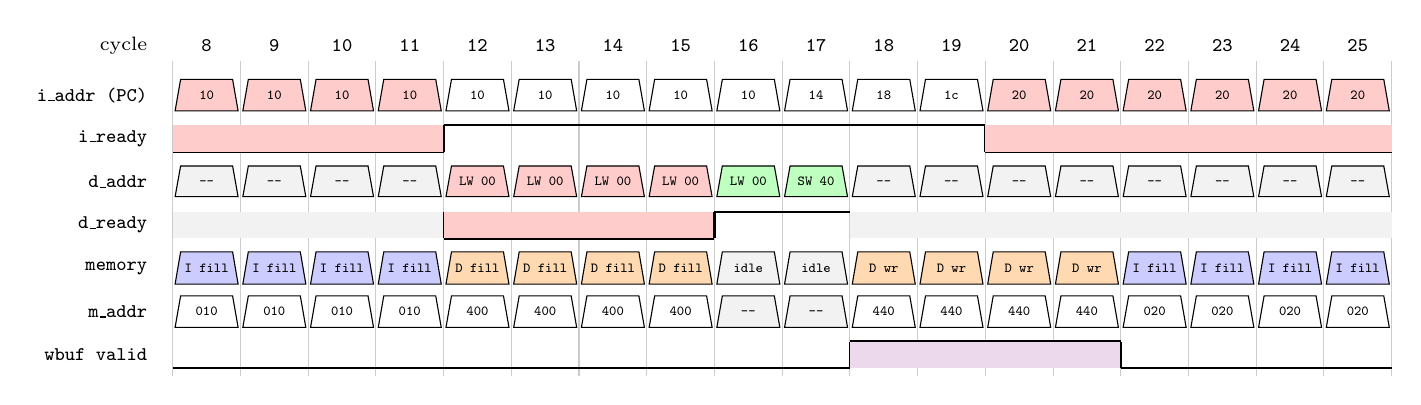
\begin{tikzpicture}[font=\scriptsize\ttfamily, x=1cm, y=1cm]
\node at (0.43,0.35) {8};
\node at (1.29,0.35) {9};
\node at (2.15,0.35) {10};
\node at (3.01,0.35) {11};
\node at (3.87,0.35) {12};
\node at (4.73,0.35) {13};
\node at (5.59,0.35) {14};
\node at (6.45,0.35) {15};
\node at (7.31,0.35) {16};
\node at (8.17,0.35) {17};
\node at (9.03,0.35) {18};
\node at (9.89,0.35) {19};
\node at (10.75,0.35) {20};
\node at (11.61,0.35) {21};
\node at (12.47,0.35) {22};
\node at (13.33,0.35) {23};
\node at (14.19,0.35) {24};
\node at (15.05,0.35) {25};
\node[anchor=east] at (-0.2,0.35) {\normalfont cycle};
\draw[gray!40] (0.00,0.15) -- (0.00,-3.85);
\draw[gray!40] (0.86,0.15) -- (0.86,-3.85);
\draw[gray!40] (1.72,0.15) -- (1.72,-3.85);
\draw[gray!40] (2.58,0.15) -- (2.58,-3.85);
\draw[gray!40] (3.44,0.15) -- (3.44,-3.85);
\draw[gray!40] (4.30,0.15) -- (4.30,-3.85);
\draw[gray!40] (5.16,0.15) -- (5.16,-3.85);
\draw[gray!40] (6.02,0.15) -- (6.02,-3.85);
\draw[gray!40] (6.88,0.15) -- (6.88,-3.85);
\draw[gray!40] (7.74,0.15) -- (7.74,-3.85);
\draw[gray!40] (8.60,0.15) -- (8.60,-3.85);
\draw[gray!40] (9.46,0.15) -- (9.46,-3.85);
\draw[gray!40] (10.32,0.15) -- (10.32,-3.85);
\draw[gray!40] (11.18,0.15) -- (11.18,-3.85);
\draw[gray!40] (12.04,0.15) -- (12.04,-3.85);
\draw[gray!40] (12.90,0.15) -- (12.90,-3.85);
\draw[gray!40] (13.76,0.15) -- (13.76,-3.85);
\draw[gray!40] (14.62,0.15) -- (14.62,-3.85);
\draw[gray!40] (15.48,0.15) -- (15.48,-3.85);
\node[anchor=east] at (-0.2,-0.28) {i\_addr (PC)};
\draw[fill=red!20] (0.03,-0.48) -- (0.10,-0.08) -- (0.76,-0.08) -- (0.83,-0.48) -- cycle;
\node[font=\tiny\ttfamily] at (0.43,-0.28) {10};
\draw[fill=red!20] (0.89,-0.48) -- (0.96,-0.08) -- (1.62,-0.08) -- (1.69,-0.48) -- cycle;
\node[font=\tiny\ttfamily] at (1.29,-0.28) {10};
\draw[fill=red!20] (1.75,-0.48) -- (1.82,-0.08) -- (2.48,-0.08) -- (2.55,-0.48) -- cycle;
\node[font=\tiny\ttfamily] at (2.15,-0.28) {10};
\draw[fill=red!20] (2.61,-0.48) -- (2.68,-0.08) -- (3.34,-0.08) -- (3.41,-0.48) -- cycle;
\node[font=\tiny\ttfamily] at (3.01,-0.28) {10};
\draw[fill=white] (3.47,-0.48) -- (3.54,-0.08) -- (4.20,-0.08) -- (4.27,-0.48) -- cycle;
\node[font=\tiny\ttfamily] at (3.87,-0.28) {10};
\draw[fill=white] (4.33,-0.48) -- (4.40,-0.08) -- (5.06,-0.08) -- (5.13,-0.48) -- cycle;
\node[font=\tiny\ttfamily] at (4.73,-0.28) {10};
\draw[fill=white] (5.19,-0.48) -- (5.26,-0.08) -- (5.92,-0.08) -- (5.99,-0.48) -- cycle;
\node[font=\tiny\ttfamily] at (5.59,-0.28) {10};
\draw[fill=white] (6.05,-0.48) -- (6.12,-0.08) -- (6.78,-0.08) -- (6.85,-0.48) -- cycle;
\node[font=\tiny\ttfamily] at (6.45,-0.28) {10};
\draw[fill=white] (6.91,-0.48) -- (6.98,-0.08) -- (7.64,-0.08) -- (7.71,-0.48) -- cycle;
\node[font=\tiny\ttfamily] at (7.31,-0.28) {10};
\draw[fill=white] (7.77,-0.48) -- (7.84,-0.08) -- (8.50,-0.08) -- (8.57,-0.48) -- cycle;
\node[font=\tiny\ttfamily] at (8.17,-0.28) {14};
\draw[fill=white] (8.63,-0.48) -- (8.70,-0.08) -- (9.36,-0.08) -- (9.43,-0.48) -- cycle;
\node[font=\tiny\ttfamily] at (9.03,-0.28) {18};
\draw[fill=white] (9.49,-0.48) -- (9.56,-0.08) -- (10.22,-0.08) -- (10.29,-0.48) -- cycle;
\node[font=\tiny\ttfamily] at (9.89,-0.28) {1c};
\draw[fill=red!20] (10.35,-0.48) -- (10.42,-0.08) -- (11.08,-0.08) -- (11.15,-0.48) -- cycle;
\node[font=\tiny\ttfamily] at (10.75,-0.28) {20};
\draw[fill=red!20] (11.21,-0.48) -- (11.28,-0.08) -- (11.94,-0.08) -- (12.01,-0.48) -- cycle;
\node[font=\tiny\ttfamily] at (11.61,-0.28) {20};
\draw[fill=red!20] (12.07,-0.48) -- (12.14,-0.08) -- (12.80,-0.08) -- (12.87,-0.48) -- cycle;
\node[font=\tiny\ttfamily] at (12.47,-0.28) {20};
\draw[fill=red!20] (12.93,-0.48) -- (13.00,-0.08) -- (13.66,-0.08) -- (13.73,-0.48) -- cycle;
\node[font=\tiny\ttfamily] at (13.33,-0.28) {20};
\draw[fill=red!20] (13.79,-0.48) -- (13.86,-0.08) -- (14.52,-0.08) -- (14.59,-0.48) -- cycle;
\node[font=\tiny\ttfamily] at (14.19,-0.28) {20};
\draw[fill=red!20] (14.65,-0.48) -- (14.72,-0.08) -- (15.38,-0.08) -- (15.45,-0.48) -- cycle;
\node[font=\tiny\ttfamily] at (15.05,-0.28) {20};
\node[anchor=east] at (-0.2,-0.83) {i\_ready};
\draw[thick] (0.00,-1.00) -- (0.86,-1.00);
\fill[red!20] (0.00,-1.00) rectangle (0.86,-0.66);
\draw[thick] (0.86,-1.00) -- (1.72,-1.00);
\fill[red!20] (0.86,-1.00) rectangle (1.72,-0.66);
\draw[thick] (1.72,-1.00) -- (2.58,-1.00);
\fill[red!20] (1.72,-1.00) rectangle (2.58,-0.66);
\draw[thick] (2.58,-1.00) -- (3.44,-1.00);
\fill[red!20] (2.58,-1.00) rectangle (3.44,-0.66);
\draw[thick] (3.44,-0.66) -- (4.30,-0.66);
\draw[thick] (3.44,-1.00) -- (3.44,-0.66);
\draw[thick] (4.30,-0.66) -- (5.16,-0.66);
\draw[thick] (5.16,-0.66) -- (6.02,-0.66);
\draw[thick] (6.02,-0.66) -- (6.88,-0.66);
\draw[thick] (6.88,-0.66) -- (7.74,-0.66);
\draw[thick] (7.74,-0.66) -- (8.60,-0.66);
\draw[thick] (8.60,-0.66) -- (9.46,-0.66);
\draw[thick] (9.46,-0.66) -- (10.32,-0.66);
\draw[thick] (10.32,-1.00) -- (11.18,-1.00);
\draw[thick] (10.32,-1.00) -- (10.32,-0.66);
\fill[red!20] (10.32,-1.00) rectangle (11.18,-0.66);
\draw[thick] (11.18,-1.00) -- (12.04,-1.00);
\fill[red!20] (11.18,-1.00) rectangle (12.04,-0.66);
\draw[thick] (12.04,-1.00) -- (12.90,-1.00);
\fill[red!20] (12.04,-1.00) rectangle (12.90,-0.66);
\draw[thick] (12.90,-1.00) -- (13.76,-1.00);
\fill[red!20] (12.90,-1.00) rectangle (13.76,-0.66);
\draw[thick] (13.76,-1.00) -- (14.62,-1.00);
\fill[red!20] (13.76,-1.00) rectangle (14.62,-0.66);
\draw[thick] (14.62,-1.00) -- (15.48,-1.00);
\fill[red!20] (14.62,-1.00) rectangle (15.48,-0.66);
\node[anchor=east] at (-0.2,-1.38) {d\_addr};
\draw[fill=gray!10] (0.03,-1.57) -- (0.10,-1.18) -- (0.76,-1.18) -- (0.83,-1.57) -- cycle;
\node[font=\tiny\ttfamily] at (0.43,-1.38) {--};
\draw[fill=gray!10] (0.89,-1.57) -- (0.96,-1.18) -- (1.62,-1.18) -- (1.69,-1.57) -- cycle;
\node[font=\tiny\ttfamily] at (1.29,-1.38) {--};
\draw[fill=gray!10] (1.75,-1.57) -- (1.82,-1.18) -- (2.48,-1.18) -- (2.55,-1.57) -- cycle;
\node[font=\tiny\ttfamily] at (2.15,-1.38) {--};
\draw[fill=gray!10] (2.61,-1.57) -- (2.68,-1.18) -- (3.34,-1.18) -- (3.41,-1.57) -- cycle;
\node[font=\tiny\ttfamily] at (3.01,-1.38) {--};
\draw[fill=red!20] (3.47,-1.57) -- (3.54,-1.18) -- (4.20,-1.18) -- (4.27,-1.57) -- cycle;
\node[font=\tiny\ttfamily] at (3.87,-1.38) {LW~00};
\draw[fill=red!20] (4.33,-1.57) -- (4.40,-1.18) -- (5.06,-1.18) -- (5.13,-1.57) -- cycle;
\node[font=\tiny\ttfamily] at (4.73,-1.38) {LW~00};
\draw[fill=red!20] (5.19,-1.57) -- (5.26,-1.18) -- (5.92,-1.18) -- (5.99,-1.57) -- cycle;
\node[font=\tiny\ttfamily] at (5.59,-1.38) {LW~00};
\draw[fill=red!20] (6.05,-1.57) -- (6.12,-1.18) -- (6.78,-1.18) -- (6.85,-1.57) -- cycle;
\node[font=\tiny\ttfamily] at (6.45,-1.38) {LW~00};
\draw[fill=green!25] (6.91,-1.57) -- (6.98,-1.18) -- (7.64,-1.18) -- (7.71,-1.57) -- cycle;
\node[font=\tiny\ttfamily] at (7.31,-1.38) {LW~00};
\draw[fill=green!25] (7.77,-1.57) -- (7.84,-1.18) -- (8.50,-1.18) -- (8.57,-1.57) -- cycle;
\node[font=\tiny\ttfamily] at (8.17,-1.38) {SW~40};
\draw[fill=gray!10] (8.63,-1.57) -- (8.70,-1.18) -- (9.36,-1.18) -- (9.43,-1.57) -- cycle;
\node[font=\tiny\ttfamily] at (9.03,-1.38) {--};
\draw[fill=gray!10] (9.49,-1.57) -- (9.56,-1.18) -- (10.22,-1.18) -- (10.29,-1.57) -- cycle;
\node[font=\tiny\ttfamily] at (9.89,-1.38) {--};
\draw[fill=gray!10] (10.35,-1.57) -- (10.42,-1.18) -- (11.08,-1.18) -- (11.15,-1.57) -- cycle;
\node[font=\tiny\ttfamily] at (10.75,-1.38) {--};
\draw[fill=gray!10] (11.21,-1.57) -- (11.28,-1.18) -- (11.94,-1.18) -- (12.01,-1.57) -- cycle;
\node[font=\tiny\ttfamily] at (11.61,-1.38) {--};
\draw[fill=gray!10] (12.07,-1.57) -- (12.14,-1.18) -- (12.80,-1.18) -- (12.87,-1.57) -- cycle;
\node[font=\tiny\ttfamily] at (12.47,-1.38) {--};
\draw[fill=gray!10] (12.93,-1.57) -- (13.00,-1.18) -- (13.66,-1.18) -- (13.73,-1.57) -- cycle;
\node[font=\tiny\ttfamily] at (13.33,-1.38) {--};
\draw[fill=gray!10] (13.79,-1.57) -- (13.86,-1.18) -- (14.52,-1.18) -- (14.59,-1.57) -- cycle;
\node[font=\tiny\ttfamily] at (14.19,-1.38) {--};
\draw[fill=gray!10] (14.65,-1.57) -- (14.72,-1.18) -- (15.38,-1.18) -- (15.45,-1.57) -- cycle;
\node[font=\tiny\ttfamily] at (15.05,-1.38) {--};
\node[anchor=east] at (-0.2,-1.93) {d\_ready};
\fill[gray!10] (0.00,-2.10) rectangle (0.86,-1.76);
\fill[gray!10] (0.86,-2.10) rectangle (1.72,-1.76);
\fill[gray!10] (1.72,-2.10) rectangle (2.58,-1.76);
\fill[gray!10] (2.58,-2.10) rectangle (3.44,-1.76);
\draw[thick] (3.44,-2.10) -- (4.30,-2.10);
\draw[thick] (3.44,-2.10) -- (3.44,-1.76);
\fill[red!20] (3.44,-2.10) rectangle (4.30,-1.76);
\draw[thick] (4.30,-2.10) -- (5.16,-2.10);
\fill[red!20] (4.30,-2.10) rectangle (5.16,-1.76);
\draw[thick] (5.16,-2.10) -- (6.02,-2.10);
\fill[red!20] (5.16,-2.10) rectangle (6.02,-1.76);
\draw[thick] (6.02,-2.10) -- (6.88,-2.10);
\fill[red!20] (6.02,-2.10) rectangle (6.88,-1.76);
\draw[thick] (6.88,-1.76) -- (7.74,-1.76);
\draw[thick] (6.88,-2.10) -- (6.88,-1.76);
\draw[thick] (7.74,-1.76) -- (8.60,-1.76);
\fill[gray!10] (8.60,-2.10) rectangle (9.46,-1.76);
\fill[gray!10] (9.46,-2.10) rectangle (10.32,-1.76);
\fill[gray!10] (10.32,-2.10) rectangle (11.18,-1.76);
\fill[gray!10] (11.18,-2.10) rectangle (12.04,-1.76);
\fill[gray!10] (12.04,-2.10) rectangle (12.90,-1.76);
\fill[gray!10] (12.90,-2.10) rectangle (13.76,-1.76);
\fill[gray!10] (13.76,-2.10) rectangle (14.62,-1.76);
\fill[gray!10] (14.62,-2.10) rectangle (15.48,-1.76);
\node[anchor=east] at (-0.2,-2.48) {memory};
\draw[fill=blue!20] (0.03,-2.68) -- (0.10,-2.27) -- (0.76,-2.27) -- (0.83,-2.68) -- cycle;
\node[font=\tiny\ttfamily] at (0.43,-2.48) {I fill};
\draw[fill=blue!20] (0.89,-2.68) -- (0.96,-2.27) -- (1.62,-2.27) -- (1.69,-2.68) -- cycle;
\node[font=\tiny\ttfamily] at (1.29,-2.48) {I fill};
\draw[fill=blue!20] (1.75,-2.68) -- (1.82,-2.27) -- (2.48,-2.27) -- (2.55,-2.68) -- cycle;
\node[font=\tiny\ttfamily] at (2.15,-2.48) {I fill};
\draw[fill=blue!20] (2.61,-2.68) -- (2.68,-2.27) -- (3.34,-2.27) -- (3.41,-2.68) -- cycle;
\node[font=\tiny\ttfamily] at (3.01,-2.48) {I fill};
\draw[fill=orange!30] (3.47,-2.68) -- (3.54,-2.27) -- (4.20,-2.27) -- (4.27,-2.68) -- cycle;
\node[font=\tiny\ttfamily] at (3.87,-2.48) {D fill};
\draw[fill=orange!30] (4.33,-2.68) -- (4.40,-2.27) -- (5.06,-2.27) -- (5.13,-2.68) -- cycle;
\node[font=\tiny\ttfamily] at (4.73,-2.48) {D fill};
\draw[fill=orange!30] (5.19,-2.68) -- (5.26,-2.27) -- (5.92,-2.27) -- (5.99,-2.68) -- cycle;
\node[font=\tiny\ttfamily] at (5.59,-2.48) {D fill};
\draw[fill=orange!30] (6.05,-2.68) -- (6.12,-2.27) -- (6.78,-2.27) -- (6.85,-2.68) -- cycle;
\node[font=\tiny\ttfamily] at (6.45,-2.48) {D fill};
\draw[fill=gray!10] (6.91,-2.68) -- (6.98,-2.27) -- (7.64,-2.27) -- (7.71,-2.68) -- cycle;
\node[font=\tiny\ttfamily] at (7.31,-2.48) {idle};
\draw[fill=gray!10] (7.77,-2.68) -- (7.84,-2.27) -- (8.50,-2.27) -- (8.57,-2.68) -- cycle;
\node[font=\tiny\ttfamily] at (8.17,-2.48) {idle};
\draw[fill=orange!30] (8.63,-2.68) -- (8.70,-2.27) -- (9.36,-2.27) -- (9.43,-2.68) -- cycle;
\node[font=\tiny\ttfamily] at (9.03,-2.48) {D wr};
\draw[fill=orange!30] (9.49,-2.68) -- (9.56,-2.27) -- (10.22,-2.27) -- (10.29,-2.68) -- cycle;
\node[font=\tiny\ttfamily] at (9.89,-2.48) {D wr};
\draw[fill=orange!30] (10.35,-2.68) -- (10.42,-2.27) -- (11.08,-2.27) -- (11.15,-2.68) -- cycle;
\node[font=\tiny\ttfamily] at (10.75,-2.48) {D wr};
\draw[fill=orange!30] (11.21,-2.68) -- (11.28,-2.27) -- (11.94,-2.27) -- (12.01,-2.68) -- cycle;
\node[font=\tiny\ttfamily] at (11.61,-2.48) {D wr};
\draw[fill=blue!20] (12.07,-2.68) -- (12.14,-2.27) -- (12.80,-2.27) -- (12.87,-2.68) -- cycle;
\node[font=\tiny\ttfamily] at (12.47,-2.48) {I fill};
\draw[fill=blue!20] (12.93,-2.68) -- (13.00,-2.27) -- (13.66,-2.27) -- (13.73,-2.68) -- cycle;
\node[font=\tiny\ttfamily] at (13.33,-2.48) {I fill};
\draw[fill=blue!20] (13.79,-2.68) -- (13.86,-2.27) -- (14.52,-2.27) -- (14.59,-2.68) -- cycle;
\node[font=\tiny\ttfamily] at (14.19,-2.48) {I fill};
\draw[fill=blue!20] (14.65,-2.68) -- (14.72,-2.27) -- (15.38,-2.27) -- (15.45,-2.68) -- cycle;
\node[font=\tiny\ttfamily] at (15.05,-2.48) {I fill};
\node[anchor=east] at (-0.2,-3.03) {m\_addr};
\draw[fill=white] (0.03,-3.23) -- (0.10,-2.83) -- (0.76,-2.83) -- (0.83,-3.23) -- cycle;
\node[font=\tiny\ttfamily] at (0.43,-3.03) {010};
\draw[fill=white] (0.89,-3.23) -- (0.96,-2.83) -- (1.62,-2.83) -- (1.69,-3.23) -- cycle;
\node[font=\tiny\ttfamily] at (1.29,-3.03) {010};
\draw[fill=white] (1.75,-3.23) -- (1.82,-2.83) -- (2.48,-2.83) -- (2.55,-3.23) -- cycle;
\node[font=\tiny\ttfamily] at (2.15,-3.03) {010};
\draw[fill=white] (2.61,-3.23) -- (2.68,-2.83) -- (3.34,-2.83) -- (3.41,-3.23) -- cycle;
\node[font=\tiny\ttfamily] at (3.01,-3.03) {010};
\draw[fill=white] (3.47,-3.23) -- (3.54,-2.83) -- (4.20,-2.83) -- (4.27,-3.23) -- cycle;
\node[font=\tiny\ttfamily] at (3.87,-3.03) {400};
\draw[fill=white] (4.33,-3.23) -- (4.40,-2.83) -- (5.06,-2.83) -- (5.13,-3.23) -- cycle;
\node[font=\tiny\ttfamily] at (4.73,-3.03) {400};
\draw[fill=white] (5.19,-3.23) -- (5.26,-2.83) -- (5.92,-2.83) -- (5.99,-3.23) -- cycle;
\node[font=\tiny\ttfamily] at (5.59,-3.03) {400};
\draw[fill=white] (6.05,-3.23) -- (6.12,-2.83) -- (6.78,-2.83) -- (6.85,-3.23) -- cycle;
\node[font=\tiny\ttfamily] at (6.45,-3.03) {400};
\draw[fill=gray!10] (6.91,-3.23) -- (6.98,-2.83) -- (7.64,-2.83) -- (7.71,-3.23) -- cycle;
\node[font=\tiny\ttfamily] at (7.31,-3.03) {--};
\draw[fill=gray!10] (7.77,-3.23) -- (7.84,-2.83) -- (8.50,-2.83) -- (8.57,-3.23) -- cycle;
\node[font=\tiny\ttfamily] at (8.17,-3.03) {--};
\draw[fill=white] (8.63,-3.23) -- (8.70,-2.83) -- (9.36,-2.83) -- (9.43,-3.23) -- cycle;
\node[font=\tiny\ttfamily] at (9.03,-3.03) {440};
\draw[fill=white] (9.49,-3.23) -- (9.56,-2.83) -- (10.22,-2.83) -- (10.29,-3.23) -- cycle;
\node[font=\tiny\ttfamily] at (9.89,-3.03) {440};
\draw[fill=white] (10.35,-3.23) -- (10.42,-2.83) -- (11.08,-2.83) -- (11.15,-3.23) -- cycle;
\node[font=\tiny\ttfamily] at (10.75,-3.03) {440};
\draw[fill=white] (11.21,-3.23) -- (11.28,-2.83) -- (11.94,-2.83) -- (12.01,-3.23) -- cycle;
\node[font=\tiny\ttfamily] at (11.61,-3.03) {440};
\draw[fill=white] (12.07,-3.23) -- (12.14,-2.83) -- (12.80,-2.83) -- (12.87,-3.23) -- cycle;
\node[font=\tiny\ttfamily] at (12.47,-3.03) {020};
\draw[fill=white] (12.93,-3.23) -- (13.00,-2.83) -- (13.66,-2.83) -- (13.73,-3.23) -- cycle;
\node[font=\tiny\ttfamily] at (13.33,-3.03) {020};
\draw[fill=white] (13.79,-3.23) -- (13.86,-2.83) -- (14.52,-2.83) -- (14.59,-3.23) -- cycle;
\node[font=\tiny\ttfamily] at (14.19,-3.03) {020};
\draw[fill=white] (14.65,-3.23) -- (14.72,-2.83) -- (15.38,-2.83) -- (15.45,-3.23) -- cycle;
\node[font=\tiny\ttfamily] at (15.05,-3.03) {020};
\node[anchor=east] at (-0.2,-3.58) {wbuf valid};
\draw[thick] (0.00,-3.75) -- (0.86,-3.75);
\draw[thick] (0.86,-3.75) -- (1.72,-3.75);
\draw[thick] (1.72,-3.75) -- (2.58,-3.75);
\draw[thick] (2.58,-3.75) -- (3.44,-3.75);
\draw[thick] (3.44,-3.75) -- (4.30,-3.75);
\draw[thick] (4.30,-3.75) -- (5.16,-3.75);
\draw[thick] (5.16,-3.75) -- (6.02,-3.75);
\draw[thick] (6.02,-3.75) -- (6.88,-3.75);
\draw[thick] (6.88,-3.75) -- (7.74,-3.75);
\draw[thick] (7.74,-3.75) -- (8.60,-3.75);
\draw[thick] (8.60,-3.41) -- (9.46,-3.41);
\draw[thick] (8.60,-3.75) -- (8.60,-3.41);
\fill[violet!15] (8.60,-3.75) rectangle (9.46,-3.41);
\draw[thick] (9.46,-3.41) -- (10.32,-3.41);
\fill[violet!15] (9.46,-3.75) rectangle (10.32,-3.41);
\draw[thick] (10.32,-3.41) -- (11.18,-3.41);
\fill[violet!15] (10.32,-3.75) rectangle (11.18,-3.41);
\draw[thick] (11.18,-3.41) -- (12.04,-3.41);
\fill[violet!15] (11.18,-3.75) rectangle (12.04,-3.41);
\draw[thick] (12.04,-3.75) -- (12.90,-3.75);
\draw[thick] (12.04,-3.75) -- (12.04,-3.41);
\draw[thick] (12.90,-3.75) -- (13.76,-3.75);
\draw[thick] (13.76,-3.75) -- (14.62,-3.75);
\draw[thick] (14.62,-3.75) -- (15.48,-3.75);
\end{tikzpicture}

\caption{Phase II, modified Harvard with $L=4$ and 8+8 lines: \texttt{memcopy}, cycles 8--25, generated from simulation. Red: the core waits (I- or D-cache miss). Green: a data access completes in the same cycle as a fetch. ``memory'' shows who owns the shared memory: I-cache fill, D-cache fill, or write-buffer drain (D wr).}
\label{fig:wavehier}
\end{figure*}

\subsection{Effect of memory latency}
Fig.~\ref{fig:latency} shows the geometric-mean CPI of the eight programs as
the latency of the shared memory grows from one to 16 cycles. Without a cache
(NC), every fetch and every data access pays the full latency, so CPI grows
linearly with $L$, from 1.21 (exactly the Phase~I baseline, as the testbench
checks) to 18.8. Caches hide most of this: at $L=16$ the split caches reach a
CPI of 3.03, a 6.2$\times$ improvement over no cache, and the unified cache
4.45. At $L=1$ the split caches (1.11) are slower than the ideal Harvard
design only by their compulsory misses, which cost one cycle each because
the refill word is not forwarded. Their CPI is already lower than that of
the ideal shared-memory machine (1.21): with split caches, the extra cycle of
every load and store disappears.

\begin{figure}[t]
\centering
% CPI vs memory latency, data from report/data/latency.dat (written by tools/sweep.py)
\begin{tikzpicture}
\begin{axis}[
    width=\columnwidth, height=5.0cm,
    xmode=log, log basis x=2, ymode=log,
    xtick={1,2,4,8,16}, xticklabels={1,2,4,8,16},
    ytick={1,1.5,2,3,5,10,20}, yticklabels={1,1.5,2,3,5,10,20},
    ymin=0.9, ymax=22,
    xlabel={Lower-level memory latency $L$ (cycles)},
    ylabel={Geometric-mean CPI (8 programs)},
    grid=major, grid style={gray!25},
    tick label style={font=\scriptsize}, label style={font=\footnotesize},
    legend style={font=\scriptsize, at={(0.5,-0.3)}, anchor=north, legend columns=2, cells={anchor=west}},
    every axis plot/.append style={thick, mark size=1.6pt}]
\addplot[black!60, dashed, mark=none]     table[x=L, y=H]  {data/latency.dat}; \addlegendentry{H: ideal Harvard}
\addplot[black!60, dotted, mark=none]     table[x=L, y=VN] {data/latency.dat}; \addlegendentry{VN: ideal shared memory}
\addplot[red!75!black, mark=triangle*]    table[x=L, y=NC] {data/latency.dat}; \addlegendentry{NC: shared memory, no cache}
\addplot[orange!85!black, mark=square*]   table[x=L, y=UC] {data/latency.dat}; \addlegendentry{UC: unified cache 16 lines}
\addplot[blue!75!black, mark=*]           table[x=L, y=MH] {data/latency.dat}; \addlegendentry{MH: split caches 8+8 lines}
\end{axis}
\end{tikzpicture}

\caption{Geometric-mean CPI of the eight programs versus the latency of the shared lower-level memory (cache lines of four words; split 8+8 lines, unified 16 lines).}
\label{fig:latency}
\end{figure}

\subsection{Split versus unified caches}
Table~\ref{tab:split} compares the two hierarchies at $L=4$ with the same
total capacity of 64 words. The split caches are faster on every program, by
1.01$\times$ (\texttt{count\_loop}) to 2.29$\times$ (\texttt{bubble\_sort}),
and by 1.38$\times$ in the geometric mean. Two effects add up. The first is
the one measured in Phase~I: even when every access hits, the unified cache
has one port, so a load or store costs an extra cycle. The second is
conflict misses. In the split design, the instruction and data streams never
evict each other, so MH takes only compulsory misses (69 in total over all
programs). In the unified cache, code starts at physical address
\texttt{0x000} and data at \texttt{0x400}. Both are multiples of the cache
size (256 bytes), so code word $k$ and data word $k$ map to the same line.
In \texttt{bubble\_sort} the loop body and the array both start at line~0,
so each load evicts the instruction line that the next fetch needs, and back:
252 misses against 10 for the split caches. This is the classic
direct-mapped conflict of Hill and Smith~\cite{hill1989}, and it would shrink
with associativity, a victim cache~\cite{jouppi1990}, or a data segment that
does not start at a multiple of the cache size.

\begin{table}[t]
\caption{Split (8+8 lines) vs.\ unified (16 lines) caches, $L=4$: CPI and misses}
\label{tab:split}
\centering
\setlength{\tabcolsep}{2.6pt}
\begin{tabular}{lrrrrrrr}
\toprule
Program & MH & UC & NC & \multicolumn{2}{c}{MH misses} & UC & MH vs. \\
 & CPI & CPI & CPI & I & D & misses & UC \\
\midrule
basic        & 2.53 & 2.79 & 4.84 &  5 &  1 &   6 & 1.10$\times$ \\
array\_sum   & 1.53 & 3.37 & 4.97 &  3 &  2 &  19 & 2.21$\times$ \\
memcopy      & 1.41 & 2.24 & 5.20 &  3 &  2 &  12 & 1.59$\times$ \\
count\_loop  & 1.12 & 1.14 & 4.02 &  2 &  0 &   2 & 1.01$\times$ \\
isa\_test    & 2.29 & 2.45 & 4.45 & 10 &  0 &  10 & 1.07$\times$ \\
bubble\_sort & 1.28 & 2.93 & 5.78 &  6 &  4 & 252 & 2.29$\times$ \\
func\_call   & 1.09 & 1.13 & 4.15 &  6 &  0 &   6 & 1.04$\times$ \\
transpose    & 1.13 & 1.46 & 4.71 &  7 & 18 &  48 & 1.29$\times$ \\
\midrule
geo.\ mean   & 1.47 & 2.03 & 4.74 & \multicolumn{3}{c}{} & 1.38$\times$ \\
\bottomrule
\end{tabular}
\end{table}

Fig.~\ref{fig:size} varies the capacity. With the smallest caches (one line
per split cache, two unified lines), the unified cache is slightly faster
(CPI 2.65 vs.\ 2.77), and at 16 words it has fewer misses (451 vs.\ 590),
because it can give more of its tiny capacity to whichever stream needs it.
This is the miss-ratio advantage of unified caches described by
Smith~\cite{smith1982}. It disappears as soon as the working sets fit: from 32
words on the split caches are clearly faster, and from 64 words on both curves are
flat. The split caches then see only compulsory misses, while the unified
cache keeps its 355 misses at every size we tried, because the code/data
aliasing described above does not depend on capacity as long as the cache
is no larger than the 1\,KB distance between the two segments.

\begin{figure}[t]
\centering
% CPI vs cache capacity at L = 4, data from report/data/size.dat (written by tools/sweep.py)
\begin{tikzpicture}
\begin{axis}[
    width=\columnwidth, height=4.8cm,
    xmode=log, log basis x=2,
    xtick={8,16,32,64,128,256}, xticklabels={8,16,32,64,128,256},
    ymin=1.0, ymax=3.0,
    xlabel={Total level-1 capacity (words): split $n+n$ lines vs.\ unified $2n$ lines},
    ylabel={Geo-mean CPI, $L=4$},
    grid=major, grid style={gray!25},
    tick label style={font=\scriptsize}, label style={font=\footnotesize},
    legend style={font=\scriptsize, at={(0.98,0.98)}, anchor=north east, cells={anchor=west}},
    every axis plot/.append style={thick, mark size=1.6pt}]
\addplot[orange!85!black, mark=square*] table[x=words, y=UC] {data/size.dat}; \addlegendentry{UC: unified cache}
\addplot[blue!75!black, mark=*]         table[x=words, y=MH] {data/size.dat}; \addlegendentry{MH: split I/D caches}
\end{axis}
\end{tikzpicture}

\caption{Geometric-mean CPI versus total level-1 capacity at $L=4$ (four-word lines).}
\label{fig:size}
\end{figure}

\subsection{Write buffer}
Table~\ref{tab:wbuf} shows MH with and without the one-entry write buffer.
Without it, a store waits the full memory latency. With it, the store
completes at once and the drain overlaps with the following instructions
(Fig.~\ref{fig:wavehier}). The buffer helps most where stores are frequent
and spread out: \texttt{func\_call} stores one result per call and improves
by 1.41$\times$ at $L=16$, \texttt{transpose} by 1.38$\times$. Bursts of
stores are limited by the buffer's single entry: in \texttt{bubble\_sort},
each swap issues two stores back to back, and 189 of its 208 data-stall
cycles at $L=4$ are the second store waiting for the first to drain. A
deeper buffer would remove most of them~\cite{jouppi1993}.

\begin{table}[t]
\caption{Modified Harvard CPI without and with the write buffer (8+8 lines)}
\label{tab:wbuf}
\centering
\setlength{\tabcolsep}{4pt}
\begin{tabular}{lrrrrr}
\toprule
Program & \multicolumn{2}{c}{$L=4$} & \multicolumn{2}{c}{$L=16$} & Gain \\
 & none & wbuf & none & wbuf & $L{=}16$ \\
\midrule
basic        & 2.58 & 2.53 & 7.63 & 7.58 & 1.01$\times$ \\
array\_sum   & 1.61 & 1.53 & 3.50 & 3.11 & 1.13$\times$ \\
memcopy      & 1.81 & 1.41 & 4.70 & 3.89 & 1.21$\times$ \\
count\_loop  & 1.12 & 1.12 & 1.50 & 1.50 & 1.00$\times$ \\
isa\_test    & 2.37 & 2.29 & 6.79 & 6.71 & 1.01$\times$ \\
bubble\_sort & 1.51 & 1.28 & 3.48 & 2.80 & 1.24$\times$ \\
func\_call   & 1.20 & 1.09 & 1.92 & 1.36 & 1.41$\times$ \\
transpose    & 1.38 & 1.13 & 2.79 & 2.02 & 1.38$\times$ \\
\bottomrule
\end{tabular}
\end{table}

\subsection{Area}
All designs were synthesized with Yosys for a Xilinx 7-series FPGA
(Table~\ref{tab:synth}). As in Phase~I, the Harvard instruction ROM was
synthesized separately with pseudo-random contents, since a ROM synthesized
together with one program lets the tool delete logic for unused
instructions. For the Phase~II systems, the lower-level memory was kept as a
black box: it stands for block RAM or off-chip memory and is identical in
both systems, so the numbers are the cost of the core and the level-1
hierarchy. With ideal memories, the Harvard system uses 20\% fewer LUTs and
33 fewer flip-flops than the shared-memory baseline (the latched instruction
register and the state bit); the baseline pays for a 512-word memory, the
two-state controller and the address multiplexing in front of its single
port. The extended instruction set made both cores larger than in Phase~I,
where the difference was 34\%. With caches, the split hierarchy again uses
about 20\% fewer LUTs than the unified one, for practically the same number
of flip-flops. Most of these flip-flops are the cache data arrays (two
$32\times32$-bit arrays, or one $64\times32$): because a refill writes four
words in one cycle, Yosys cannot map them to LUT-RAM. These are synthesis
estimates; the maximum clock frequency needs Vivado place-and-route and was
not measured.

\begin{table}[t]
\caption{Yosys synthesis, Xilinx 7-series (memcopy images)}
\label{tab:synth}
\centering
\setlength{\tabcolsep}{3pt}
\begin{tabular}{lrrrr}
\toprule
Design & Logic & LUT-RAM & Total & Flip- \\
 & LUTs & LUTs & LUTs & flops \\
\midrule
H: core, data side, counters   &  761 & 176 &  937 &  194 \\
H: instruction ROM            &  128 &   0 &  128 &    0 \\
\textbf{H total}              & \textbf{889} & \textbf{176} & \textbf{1065} & \textbf{194} \\
\textbf{VN total}             & \textbf{1032} & \textbf{304} & \textbf{1336} & \textbf{227} \\
\midrule
\textbf{MH}: core + I/D caches + arbiter & \textbf{3864} & \textbf{56} & \textbf{3920} & \textbf{2520} \\
\textbf{UC}: core + unified cache       & \textbf{4833} & \textbf{52} & \textbf{4885} & \textbf{2452} \\
memory model (not in MH/UC)    &  653 & 1408 & 2061 &    8 \\
\bottomrule
\end{tabular}
\end{table}

\subsection{Limitations}
The results should be read with the model's simplifications in mind. The
lower-level memory has a fixed latency and returns a whole line in one
transfer; a real DRAM has variable latency and a narrower bus. The core is
single-cycle and not pipelined, so it cannot overlap a miss with useful
work, which makes stalls more expensive than in a pipelined core. The
programs are small kernels whose working sets fit in 64 words, which is why
the curves in Fig.~\ref{fig:size} flatten early. And the unified-cache
penalty depends on our choice of a 1\,KB distance between code and data, a
common but not universal layout.

% =============================================================================
\section{Individual Contributions}

Table~\ref{tab:contrib} summarises who built what across both phases. Every
entry corresponds to commits by that member in the project repository.

\begin{table*}[t]
\caption{Individual contributions}
\label{tab:contrib}
\centering
\small
\setlength{\tabcolsep}{4pt}
\begin{tabularx}{\textwidth}{@{}>{\raggedright\arraybackslash}p{0.09\textwidth}>{\raggedright\arraybackslash}p{0.15\textwidth}>{\raggedright\arraybackslash}X>{\raggedright\arraybackslash}X@{}}
\toprule
Member & Role & Phase I & Phase II \\
\midrule
\MemA & Memory subsystem & instr\_mem, data\_mem, addr\_decoder, rw\_ctrl, harvard\_mem & cache (I-, D- and unified cache, write buffer), main\_mem, cache unit testbench \\
\MemB & Processor, integration & regfile, alu, imm\_gen, control, pc\_reg, cpu\_core, harvard\_top; repository set-up & ISA extension (control, alu, imm\_gen), stall support in cpu\_core, mh\_top integration \\
\MemC & Baseline, metrics, synthesis & perf\_counters, shared\_mem, cpu\_core\_vn, vn\_top, comparison table, Yosys synthesis & mem\_arbiter, event\_counter, stall support in cpu\_core\_vn, vnc\_top, synthesis of all Phase II designs, area table \\
\MemD & Verification & assembler, programs, testbenches, Makefile, waveform figure & assembler extension, ISS golden model, four new programs, tb\_hier, parameter sweep, Phase II waveform \\
\MemE & Report, video, repository & report, figures, video script and video & final report, Phase II figures and plots, README, documentation \\
\bottomrule
\end{tabularx}
\end{table*}

\textbf{\MemA} designed the Harvard memory subsystem in Phase~I: the
read-only instruction memory, the data RAM, the address decoder with the
\texttt{out\_port} and fault regions, the read/write controller, and the
\texttt{harvard\_mem} wrapper that keeps the two ports independent. In
Phase~II \MemA{} designed the cache module used for the I-cache, the D-cache
and the unified cache, including the write-through policy, the write
buffer, the no-write-allocate rule and the uncached mode, the lower-level
memory with configurable latency, and the directed cache testbench.

\textbf{\MemB} built the single-cycle processor (register file, ALU,
immediate generator, control decoder, program counter and datapath) and the
\texttt{harvard\_top} integration in Phase~I, and set up the repository and
its interface specification. In Phase~II \MemB{} extended the instruction
set to 25 instructions, added the stall interface to the core, and
integrated the modified Harvard system \texttt{mh\_top}.

\textbf{\MemC} wrote the performance counters, the 512-word shared memory,
the two-state baseline processor and \texttt{vn\_top}, and ran the Phase~I
synthesis. In Phase~II \MemC{} wrote the memory arbiter and the event
counters, added stall support to the baseline core, built the unified-cache
system \texttt{vnc\_top}, and synthesized all Phase~II designs.

\textbf{\MemD} wrote the two-pass assembler, the four Phase~I programs, the
unit, system and comparison testbenches, the simulation Makefile and the
waveform generator in Phase~I. In Phase~II \MemD{} extended the assembler,
wrote the instruction-set simulator used as golden model, the four new
programs, the four-system testbench, the parameter sweep with its
cross-check, and the Phase~II waveform generator.

\textbf{\MemE} wrote the Phase~I report and its figures, the video script,
and edited the prototype video\footnote{Phase I video demonstration: \url{https://drive.google.com/drive/folders/1SoN0jAJ3BcboLqRUhE7eCVd88pDHP2RP?usp=sharing}}.
In Phase~II \MemE{} wrote this final report, its block diagram and plots,
and maintained the README and the project documentation.

% =============================================================================
\section{Conclusion}
\label{sec:concl}
We implemented a Harvard memory organisation and a shared-memory baseline
around the same RV32I-subset processor, and then extended both into a
realistic memory hierarchy with caches, a write buffer and a slow shared
memory. With ideal memories, separate instruction and data paths remove the
extra cycle that every load and store costs on a single port (CPI 1.00
against 1.02--1.45). With a shared memory of realistic latency, caches are
essential (6.2$\times$ at $L=16$), and keeping them split, as modern
processors do, is better than unifying them: at equal capacity the split
caches are 1.38$\times$ faster in the geometric mean, because they keep the
two ports and avoid conflict misses between code and data, and they use
about 20\% fewer LUTs. The unified cache wins only when the capacity is so
small that sharing it matters more than the second port. Everything is
verified against an independent golden model, in 104 configurations.

Natural next steps are a pipelined core, which would overlap misses with
execution; a deeper write buffer, which our \texttt{bubble\_sort} results
call for; set-associative caches or a victim cache to remove the code/data
conflicts of the unified cache; a refill of one word per cycle, so that the
cache arrays map to LUT-RAM; and implementation on an FPGA board to measure
the maximum clock frequency.

% =============================================================================
\section*{Acknowledgment}
The team used AI-assisted coding tools in their editors while writing code,
testbenches and documentation. Every member reviewed, simulated and is able to
explain the work submitted under their name; all results in this report are
taken from the simulation and synthesis logs in the repository.
% Check the course policy on AI use and adjust this wording if required.

% =============================================================================
\bibliographystyle{IEEEtran}
\bibliography{refs}

\end{document}
